% !TEX root = ../main.tex

\section{Introduction}

\subsection{Motivation}

When the Bitcoin exchange Mt. Gox was declared bankrupt in 2014, a curious fact was reported in the \textit{New York Times}---the missing 744K BTC ``had gone unnoticed for years.'' This led the Bitcoin community to propose that exchanges undergo regular financial audits, with proposals ranging from traditional audits conducted by specialists to completely disintermediated ``crypto-audits'' done directly by the exchange to its users using cryptography. Academics quickly showed these can be done in strict zero-knowledge~\cite{provisions}, and generated a stream of research papers that continues to improve efficiency~\cite{bulletproofs,zeroledge,dapol,spp,notus,izpr} and examine the correctness of deployed proofs~\cite{broken}. Despite these efforts, exchanges are not legally required to use a proof of solvency in jurisdictions today, with some exchanges opting to do them anyways and many not. Meanwhile, many other exchanges have failed in similar ways to Mt. Gox (whether by incompetence or fraud), including higher profile cases like QuadrigaCX and FTX. We argue that proofs of solvency are not perfect but do provide meaningful barriers (or friction) to fraud and incompetence. As academics, we believe we should continue refining these proofs toward practical implementation.  

% = = = = = = = = = = = = = = = = = = = = = = = = = = = = = = = = = = =

\subsection{Contributions}

A proof of solvency (or proof of reserves) is a zero-knowledge proof conducted by centralized cryptocurrency exchange (or more generally, any custodian of cryptocurrencies) to offer evidence that the exchange owns enough cryptocurrency to settle each of its users balances. The zero-knowledge component protects the exchange's proprietary information such as: number of users, balances of individual users, total balance of all users, which cryptocurrency addresses belong to the exchange, and total amount of cryptocurrency owned by the exchange. The proof itself is broken into sub-components: ($\pi_\mathsf{keys}$) a proof of knowledge of private signing keys associated with public cryptocurrency addresses (hidden in a freely-composable anonymity set of addresses not belonging to the exchange); ($\pi_\mathsf{assets}$) a summation of these assets into the total assets; ($\pi_\mathsf{user}$) an individualized proof given to each user asserting their balance as used in the overall proof; ($\pi_\mathsf{liabilities}$) a summation of these individual liabilities into the total liabilities; and ($\pi_\mathsf{solvency}$) a demonstration that the subtraction of total liabilities from the total assets is at least 0.

In our paper, we examine the extent to which these sub-components can be made succinct. In particular, we are interested in constant-sized arguments\footnote{We abuse terminology and generally do not distinguish between `proofs' and `arguments,' using the term `proofs' for both. Proofs provide soundness against unbounded malicious provers, while arguments provide zero knowledge against unbounded malicious verifiers. \Sys is a hybrid.} and constant-time verification. This is possible for general arithmetic circuits in the polynomial interactive oracle proof (Poly-IOP) model using protocols like Plonk and its variants. In reference to the ``towards'' in the title of our paper, we are not able to make each sub-component fully succinct, however we make progress as follows: ($\pi_\mathsf{assets}$,$\pi_\mathsf{user}$,$\pi_\mathsf{solvency}$) are constant in size and time (once all public inputs have been interpolated into polynomials by the verifier); ($\pi_\mathsf{keys}$) is linear in the number of addresses in the anonymity set (but is pre-computation that can be re-used when proofs are issued each day); ($\pi_\mathsf{liabilities}$) is linear in the number of bits used to represent each account balance (\eg 32 bits) and is independent of the number of users (technically there is an upper-bound, but it is beyond the reasonable size of the largest exchange).

Our contributions can be summarized as:

\begin{itemize}
\item \Sys:\footnote{Folklore creature revered in ancient Chinese culture for its ability to distinguish truth from deceit.} A mostly succinct protocol that covers every step of the proof, where each sub-component of the proof works with each other sub-component.
\item A novel technique for mapping knowledge of private keys of common blockchains, such as Bitcoin and Ethereum, from their group (\secp) into a pairing-friendly group (\bls) used for succinct arguments.
\item Practical adjustments to the protocol to account for concrete parameters, such as the maximum root of unity in \bls. 
\item Proof of concept implementation of \Sys with performance experimentation.
\end{itemize}

% = = = = = = = = = = = = = = = = = = = = = = = = = = = = = = = = = = =

\subsection{Limitations}

We do not argue that a proof of solvency is a silver bullet that prevents all fraud and insolvency. However we do believe it can meaningfully raise the bar for incompetence and fraud within an exchange, while providing a trail of records useful during a financial audit or enforcement action. Limitations of \Sys include: 

\begin{itemize}
\item Our protocol relies on a trusted setup. However the setup is universal (shareable with other zk-SNARK systems) and is secure with one honest participant in a decentralized computation of it~\cite{tau}.
\item $\pi_\mathsf{keys}$ assumes the public key (as opposed to only its hash) associated with every address in an anonymity set of keys is known. In Bitcoin and Ethereum, this (typically) corresponds to the address having originated at least one transaction. 
\item $\pi_\mathsf{keys}$ assumes funds are controlled by a single public key. We do not explore how to handle multisig, wallets, Gnosis Safe, \etc However we can support tokens (\eg ERC20, ERC721,\etc) given the mapping between balances and public keys is on-chain, and we can support such assets split across layer two solutions or EVM-chains. 
\end{itemize}

Limitations of proofs of solvency in general (not specific to \Sys) include:

\begin{itemize}
\item Proofs of solvency rely on human behaviour. It needs to be unpredictable to the exchange which users will check and report inconsistencies.
\item Proofs of solvency are a detection mechanism, not a prevention mechanism. Proofs do not help prevent hacks or exit scams. However they greatly complicate cover-ups by the exchange after fraud or a loss of funds has occured.
\item Collusion between parties to pool assets can enable an insolvent exchange to pass a proof of solvency. However the exchange is forced in this case to proactively seek and implement collusion, which raises the chances of discovery. It also goes to motive for fraud (many bankrupt exchanges argue they were just incompetent and it is difficult to distinguish). 
\item Trusted execution environments (TEEs) can reduce trust amongst colluders by sharing the ability to prove ownership without sharing the key itself. However we can adapt $\pi_\mathsf{keys}$ (the $\Sigma$-protocol inside it) for complete knowledge~\cite{completeknowledge}.
\item Demonstrably holding cryptocurrencies in an address does not mean the money is unencumbered. For example, it might be in use off-chain as collateral for a loan. 
\end{itemize}

% = = = = = = = = = = = = = = = = = = = = = = = = = = = = = = = = = = =

\section{Preliminaries}

\subsection{Accounting Terminology}

Our terminology follows the accounting and auditing literature. A balance sheet consists of liabilities (value owed to others) and assets (value owned). When total asset value is the same or more than total liabilities, the firm is called solvent. The amount by which the assets exceed the liabilities is called capital or equity (depending on context). Some literature prefers the term `proof of reserves' to `proof of solvency.' This terminology is also sound, although it is not always defined correctly: technically a reserve is an asset that cancels out a corresponding liability, both in amount and in type. A firm can be solvent but not have full reserves. Most banks operate this way with cash liabilities, some assets in cash, but most assets in loans and other investments.\footnote{Banks in the United States have reserve requirements while banks elsewhere, \eg Canada, have capital requirements. Capital requirements speak to solvency, while reserve requirements speak to reserve ratios. Banks that underwent the 2008 financial crisis were more robust when they had capital requirements, as opposed to reserve requirements.} Cryptographic protocols in the literature generally assume both liabilities and assets are the same cryptocurrency so exchanges are expected to be both solvent and have full reserves.

\subsection{Related Work}
\label{sec:rw}

% !TEX root = ../main.tex

\begin{table}[t]
\centering
\begin{tabular}{|p{2.5cm}|p{7cm}|p{2.5cm}|}
\hline

$\Sigma$-Protocols 
& The first proofs of solvency are based on $\Sigma$-Protocols which work on standard elliptic curves like \secp but are not succinct (linear proof space, linear verifier time, heavy constants). 
& Provisions~\cite{provisions} \\ \hline

Inner-product arguments 
& Protocols like bulletproofs work on standard elliptic curves like \secp and can reduce some sub-routines (e.g., range arguments) to constant space and logarithmic verifier time. 
& Bulletproofs~\cite{bulletproofs} \\ \hline

Liabilities only 
& As it is the asset-side of solvency that ties the protocol to standard elliptic curves like \secp, proving only the liability side can be done in any cryptographic setting. 
& ZeroLedge~\cite{zeroledge}, DAPOL+~\cite{dapol}, SSVT-based~\cite{spp}, Notus~\cite{notus}, SafeCex\tablefootnote{V. Buterin, ``Having a safe CEX: proof of solvency and beyond,'' \href{https://web.archive.org/web/20230919210728/https://vitalik.ca/general/2022/11/19/proof_of_solvency.html}{vitalik.ca}, 2022} \\ \hline

Publish assets 
& A trivial proof of assets is one that is not zero-knowledge. An exchange could reveal all its addresses and prove ownership by signing a proof-specific message from each address.
& Summa\tablefootnote{\url{https://summa.gitbook.io/summa}} \\ \hline

Circuit-level 
& A general zk-snark can implement any arithmetic circuit, including \secp operations, which offers a proof of constant size and constant verifier time. 
& IZPR~\cite{izpr}, Proven.tools\tablefootnote{\url{https://www.proven.tools/}} \\ \hline

Custom blockchain 
& If new blockchains are deployed, they could use digital signatures over pairing-friendly curves. 
& Mina\tablefootnote{\url{https://minaprotocol.com/}} \\ \hline

Mapping between groups 
& If \secp values can be mapped to a pairing-friendly group, Poly-IOP arguments can potentially reduce the rest of the proof to constant size and constant verifier time. 
& COPZ~\cite{chase22}, \Sys \\ \hline

\end{tabular}
\caption{How to deal with the fact that Bitcoin and Ethereum use \secp digital signatures when trying to make a succinct proof of solvency.\label{tab:rb1}}
\end{table}

%\begin{figure}[t]
%\centering
%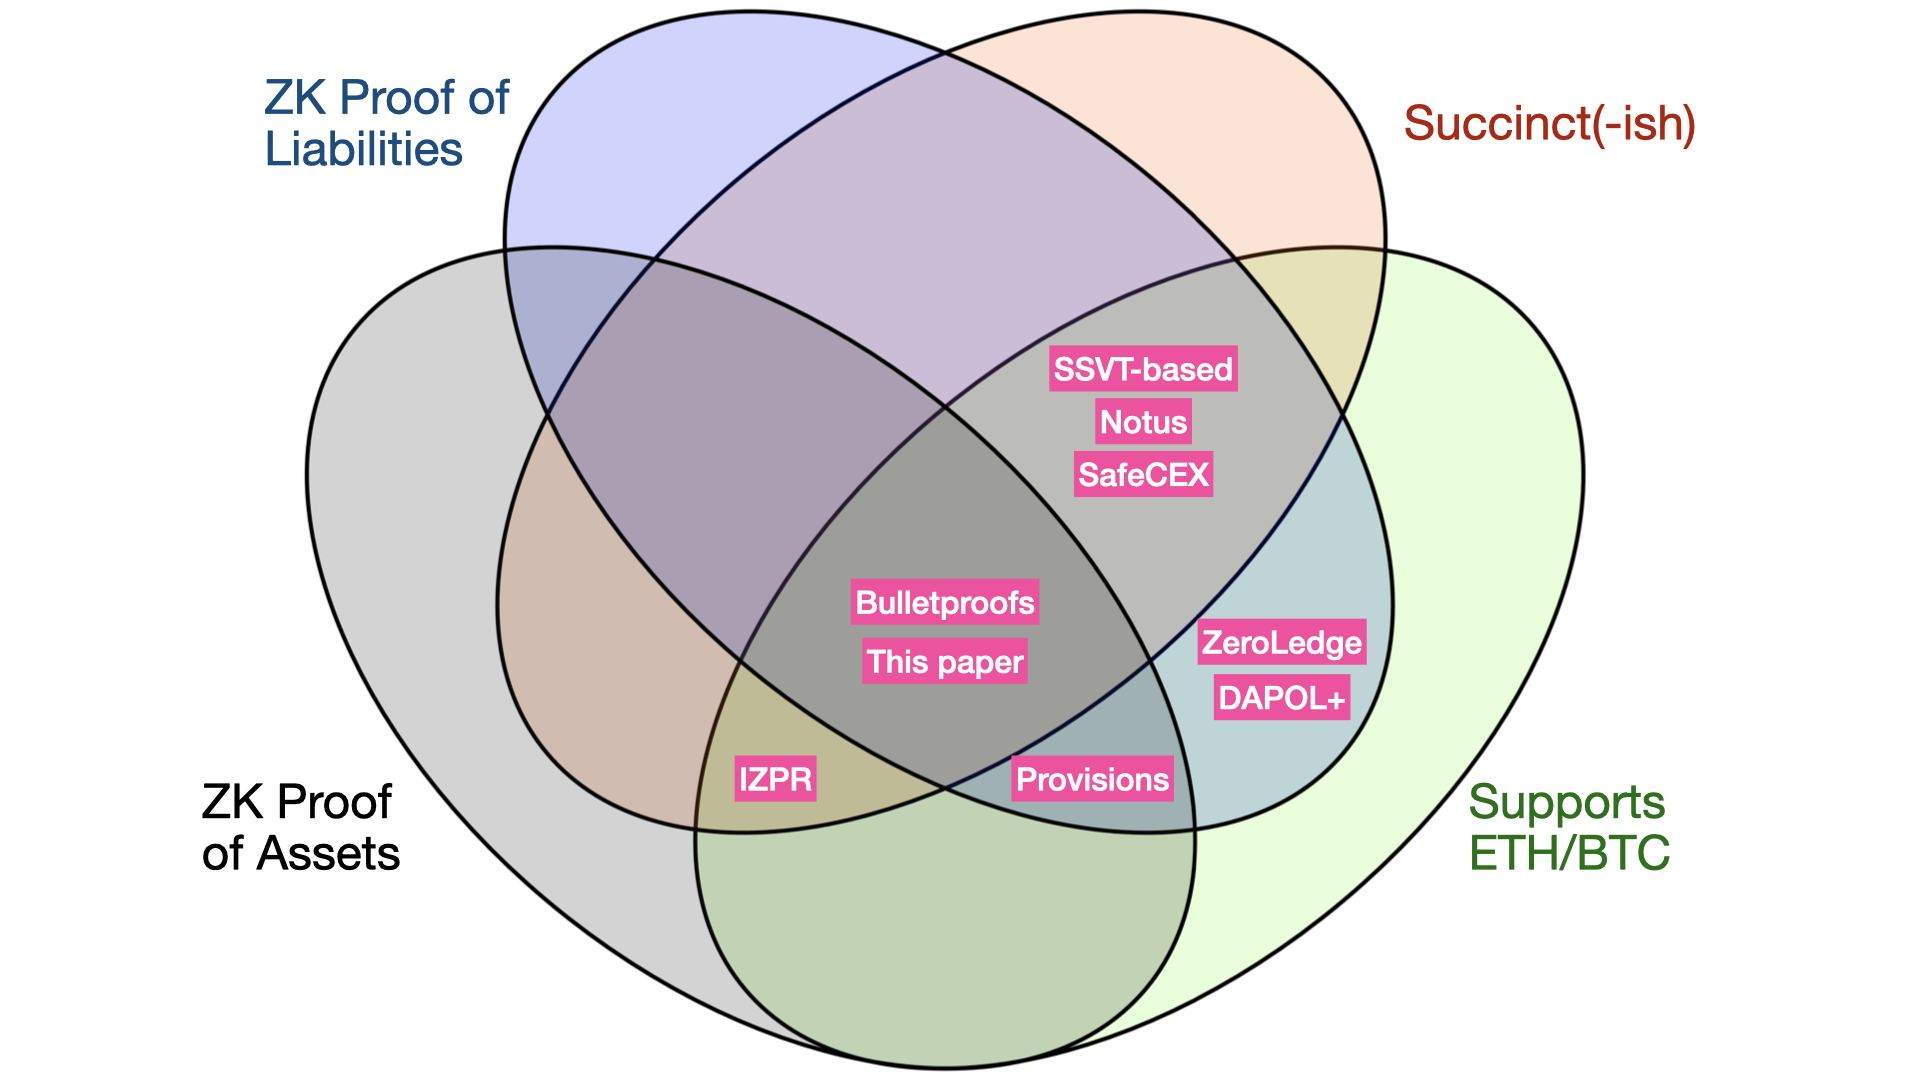
\includegraphics[width=0.8\textwidth]{figures/venn.png}
%\caption{default. \label{default}}
%\end{figure}

Proofs of solvency began as a discussion on Bitcointalk, where a protocol was developed for an exchange to announce a commitment to a total liability, and offer a Merkle-tree proof to each user that their balance was reflected in this total liability amount. Provisions, a research paper, used homomorphic commitments and $\Sigma$-protocols to add zero-knowledge, plus it added a proof of assets that could be used with the proof of liabilities to prove overall solvency~\cite{provisions}. As Provisions relies heavily on range proofs for liabilities, Bulletproofs can reduce the proof size of Provisions by 300x~\cite{bulletproofs}. Our protocol uses a polynomial-based range proof~\cite{rangeproof} to further reduce proof size and verifier time.

Outside of Provisions, Bulletproofs, and \Sys, the vast majority of work on proofs of solvency have not attempted an end-to-end proof, focusing instead on just the liabilities or just the assets. Why? We hypothesize that the biggest impediment is that Bitcoin and Ethereum assets are controlled by \secp private keys (see Table~\ref{tab:rb1}). Outside of Bulletproofs (based on inner-product arguments that do not require bilinear pairings and thus, can be implemented in \secp), most other approaches to succinctness require a specific cryptographic setting that is not \secp (\ie RSA for accumulators, pairing-based cryptography for zk-SNARKs, and lattices for zk-STARKs). If one only considers liabilities, then this problem does not have to be dealt with.

Circuit-based solutions are feasible but expensive for the prover---the authors of IZPR report about 500K constraints needed per key and proving times in the order of days for an anonymity set of 6000 keys~\cite{izpr}. By contrast, \Sys is a few minutes of work for the prover for 6000 keys. As this part is not-succinct (it is based on $\Sigma$-protocols), the trade-off is that the verifier has to do a few minutes of work as well. In both cases, IZPR and \Sys, this step does not need to be repeated often, only when the exchange wants to introduce new keys holding its assets. It is also important to recognize IZPR can let the exchange add keys it has not used yet to $\pi_{keys}$, further reducing how often this proof needs to be redone. This is a desirable property we are not able to easily achieve in \Sys (in short, it is due to our  use of selector polynomials instead of lookup arguments but future work could explore blending the best properties of \Sys and IZPR). 

% = = = = = = = = = = = = = = = = = = = = = = = = = = = = = = = = = = =

\subsection{Cryptographic Background}

\Sys is mostly a zero-knowledge argument that represents vectors of data as univariate polynomials, which are committed to and provided to the verifier. Properties of the vectors are demonstrated by manipulating the polynomials and opening points of the polynomials---a model called a polynomial interactive oracle proof (Poly-IOP). However before encoding the data into polynomials, the exchange will prove ownership of signing keys with a $\Sigma$-protocol.

We assume our protocol works in a finite field of prime order. For simplicity, we use $\prv$ and $\vrf$ to denote the prover and the verifier in an interactive proof system respectively. We use $g_\mathfrak{g}$ to denote a generator in a group $\mathbb{G}_\mathfrak{g}$ while $h_\mathfrak{g}$ is another generator, and no one knows the relative discrete logarithm of these two generators. We use $\gs$ and $\hs$ to denote the two generators in $\mathbb{G}_s$, the \secp group; and we use $\gb$ and $\hb$ to denote the two generators in $\mathbb{G}_b$, the \bls group. If we need to distinguish which group an input to the pairing is from, we use the notations $[x]_1:=g_1^x,[x]_2:=g_2^x$, otherwise elements are  assumed to be in the first group (including $g_b$ and $h_b$). We use $e([x]_1,[x]_2)$ to denote a non-degenerate bilinear pairing. We use $\hash$ to denote a collision-resilient hash function modelled as a random oracle. We use $\ppt$ to represent probabilistic algorithms run in polynomial time.  For vectors, we use an overhead bar, like $\overline{v}$, to denote a vector and brackets to denote the elements in this vector, e.g., $\overline{v}=\tuple{v_1,v_2,\dots}$. We also use a vector at the top right of a variable to indicate this variable belongs to this vector for readability, e.g., $x^{(\overline{v})}$ means $x$ is an element of $\overline{v}$. We may use these two denotations interchangeably. When we say the summation between two vectors $\overline{a},\overline{b}$, the result is a new vector $\overline{c}$ where each element is the summation of the elements from $\overline{a}$ and $\overline{b}$ at the same row.

We refer the reader to the appendix for the following cryptographic primitives: discrete logarithm assumption (Section~\ref{sec:dlp}), Pedersen commitments (Section~\ref{sec:pedersen}), $\Sigma$-protocols (conjunction and disjunction) (Section~\ref{sec:sigma}), KZG polynomial commitments (Section~\ref{sec:pcs}), and roots of unity (Section~\ref{app:rou}). We review two additional primitives here: polynomial-based range proofs and batched KZG commitments with zero-knowledge extension.

\subsubsection{Range proof}
\label{sec:range}

A range proof enables $\prv$ to convince $\vrf$ a value $x$ is in the range $[0,2^k)$ without revealing $x$. Zero-knowledge range proofs (ZKRPs) have three typical approaches: square decomposition, $n$-ary decomposition, and hash chains~\cite{zkrp}. We use the polynomial-based range proof from Boneh \etal~\cite{rangeproof}.
\begin{enumerate}
    \item \textit{Given input $x$, decompose $x$ to a vector of binary digits $\overline{z}=\tuple{z_1,z_2,\dots,z_k}$, so that $x=\sum_{i=0}^{k-1}2^i\cdot{z_i}$} 
    \item \textit{Construct a vector $\overline{x}=\tuple{x_1,x_2,\dots,x_k}$ such that}
    \begin{align*}
        x_1&=x \\
        x_k&=z_k \\
        x_i&=2x_{i+1}+z_i,i\in[1,k-1]
    \end{align*}
    \item \textit{Interpolate a polynomial $f$ from $\overline{x}$ over a finite field $H$ of order $n$ with elements $\omega^0,\omega^1,\omega^2,\ldots$ (see Appendix~\ref{app:rou})} 
    \item \textit{Prove the following polynomials are vanishing in $H$}
    \begin{align*}
        w_1&:=[f(X)-x]\cdot\frac{X^n-1}{X-\omega^0} \\
        w_2&:=f(X)\cdot[f(X)-1]\cdot\frac{X^n-1}{X-\omega^{n-1}} \\
        w_3&:=[f(X)-2\cdot{f(X\omega)}]\cdot[f(X)-2\cdot{f(X\omega)}-1]\cdot(X-\omega^{n-1})
    \end{align*}
    \begin{enumerate}
        \item $\prv$ \textit{sends the commitment to $f(X)$}
        \item $\vrf$ \textit{sends a random challenge $\gamma$}
        \item $\prv$ \textit{sends the commitment to $q(X)=w/(X^n-1)$, such that}
        \[ w=w_1+\gamma\cdot{w_2}+\gamma^2\cdot{w_3} \]
        \item $\vrf$ \textit{sends a random evaluation point $\zeta\in\mathbb{F}$}
        \item $\prv$ \textit{replies with $f(\zeta),f(\zeta\omega),q(\zeta)$}
        \item $\vrf$ \textit{checks}
        \begin{enumerate}
            \item $w(\zeta)=q(\zeta)\cdot(\zeta^n-1)$
            \item $f(\zeta),f(\zeta\omega),q(\zeta)$ \textit{are the correct evaluations}
        \end{enumerate}
    \end{enumerate}
\end{enumerate}

\subsubsection{Batched opening with zero-knowledge extension ($\open$)}
\label{sec:kgzzkp}


To efficiently prove several polynomials are vanishing at several points, there are some batched KZG opening schemes such as the schemes in \cite{plonk,bdfg,fflonk}. Although a PCS does not reveal the committed polynomial directly, it leaks the information of the opening evaluation point. In our scenario, each evaluation is privacy-sensitive so we want to hide the polynomial evaluations. We use the opening scheme from \cite{plonk} and the protocol from \cite{rangeproof} with a zero-knowledge extension to explain how to prove the range-proof polynomials are vanishing efficiently and in zero-knowledge. \\
\textit{Assume $\prv$ is given $x$ and $\vrf$ is given $[x]_1$, $\prv$ wants to prove $x$ is in $[0,2^k)$:}
\begin{enumerate}
    \item $\prv$ \textit{interpolates the polynomial $f$ using the above range proof}
    \item $\prv$ \textit{generates two random numbers $\omega^{\prime},\omega^{\prime\prime}$ in $\mathbb{F}\setminus{H}$ and another two random numbers $\alpha,\beta$ in $\mathbb{F}$}
    \item $\prv$ \textit{interpolates $f^\prime$ at two more points ${\omega^{\prime},\omega^{\prime\prime}}$ such that}
    \[ f^\prime(\omega^{\prime})=\alpha \]
    \[ f^\prime(\omega^{\prime\prime})=\beta \]
    \item $\prv$ \textit{computes $w_1,w_2,$ and $w_3$ in the above range proof and sends the commitment to $f^\prime$,} $\cm_{f^\prime}$
    \item $\vrf$ \textit{sends a random challenge $\gamma\in\mathbb{F}$}
    \item $\prv$ \textit{sends the commitment to $q_w:=w/(X^n-1)$ where}
    \[ w:=w_1+\gamma\cdot{w_2}+\gamma^2\cdot{w_3} \]
    \item $\vrf$ \textit{sends a random evaluation point $\zeta\in\mathbb{F}\setminus{H}$}
    \item $\prv$ \textit{sends the evaluations $f(\zeta),f(\zeta\omega),q_w(\zeta)$}
    \item $\prv$ \textit{sends the commitments to $q_1(X),q_2(X)$, where}
    \[ q_1(X):=\frac{f(X)-f(\zeta)}{X-\zeta}+\gamma\cdot\frac{q_w(X)-q_w(\zeta)}{X-\zeta} \]
    \[ q_2(X):=\frac{f(X)-f(\zeta\omega)}{X-\zeta\omega} \]
    \item $\vrf$ \textit{chooses random $r\in\mathbb{F}$}
    \item $\vrf$ \textit{accepts the proof if and only if}
    \begin{enumerate}
    	\item $w_1(\zeta)+\gamma\cdot{w_2(\zeta)}+\gamma^2\cdot{w_3(\zeta)}=q_w(\zeta)\cdot(\zeta^n-1)$
    	\item $e(F+\zeta\cdot\cm_{q_1}+r\zeta\cdot\cm_{q_2},[1]_2)=e(\cm_{q_1}+r\cdot\cm_{q_2},[x]_2)$\textit{, where}
    	\begin{align*}
    		F:=&\cm_f-[f(\zeta)]_1+\gamma\cdot(\cm_{q_w}-[q_w(\zeta)]_1)da+r\cdot(\cm_f-[f(\zeta\omega)]_1)
    	\end{align*}
    \end{enumerate}
%    \item $\prv$ \textit{interpolates a polynomial $g$ such that $g(\tau)=f(\tau),g(\tau\omega)=f(\tau\omega)$ and sends $g$}
%    \item $\prv$ \textit{sends the commitment to $q_{w^\prime}:=w^\prime/(X^n-1)$, where}
%    \begin{align*}
%    	w^\prime:=&(f(X)-g(X))\cdot\frac{X^n-1}{(X-\tau)(X-\tau\omega)}
%    \end{align*}
%    \item $\vrf$ \textit{sends another random evaluation point $\rho\in\mathbb{F}$}
%    \item $\prv$ \textit{sends the commitment to $q_{\hat{w}}:=\hat{w}/(x-\rho)$, where}
%    \begin{align*}
%    	\hat{w}:=&(f(X)-g(\rho))\cdot\frac{\rho^n-1}{(\rho-\tau)(\rho-\tau\omega)}-q_{w^\prime}(X)\cdot(\rho^n-1)
%    \end{align*}
%    \textit{Note $\hat{w}$ is a zero polynomial for all $x\in\mathbb{F}$, which means $X-\rho$ divides $\hat{w}$}
%    \item $\vrf$ \textit{accepts the proof if and only if}
%    	\begin{enumerate}
%    		\item $w_1(\tau)+\gamma\cdot{w_2(\tau)}+\gamma^2\cdot{w_3(\tau)}=q_w(\tau)\cdot(\tau^n-1)$
%    		\item $g(\tau)=f(\tau),g(\tau\omega)=f(\tau\omega)$
%    		\item \textit{$e(F,[1]_2)=e([q_{\hat{w}}]_1,[x-\rho]_2)$, where}
%	    		\begin{align*}
%	    		F:=&(\cm_f-[g(\rho)]_1)\cdot\frac{\rho^n-1}{(\rho-\tau)(\rho-\tau\omega)}-[q_{\hat{w}}]_1\cdot(\rho^n-1)
%	    		\end{align*}
%    	\end{enumerate}
\end{enumerate}

We prove the protocol has zero knowledge. \\
\textit{Let $\mathcal{S}$ generate $\{\omega_i^\prime,\omega_i^{\prime\prime},\alpha_i,\beta_i\},i\in[0,m]$ and interpolate $\{f_i\}$ such that}
\[ f_i(\omega_i^\prime)=\alpha_i \]
\[ f_i(\omega_i^{\prime\prime})=\beta_i \]
\[ f_i(\omega^i)=0 \]
\textit{where $i\in[0,m]$ and $\omega$ is the root of unity in $H$. Note} $\vrf$ \textit{can interact with $\mathcal{S}$ to execute the protocol and accept the proof from $\mathcal{S}$. Given $\{\omega_i^\prime,\omega_i^{\prime\prime},\alpha_i,\beta_i\}_{i\in[0,m]}$ are chosen uniformly at random each time,} $\vrf$ \textit{cannot distinguish between the transcript from $\mathcal{S}$ and the proof from} $\prv$. \textit{Therefore, the protocol has zero knowledge. We will use} $\open$ \textit{to denote this opening technique.}

% = = = = = = = = = = = = = = = = = = = = = = = = = = = = = = = = = = =

\section{Proof of Assets (PoA)}

We will begin on the asset-side of the proof of solvency. To ease the writing, we will take the example of an exchange proving solvency for ETH on Ethereum. The PoA is broken into two steps: \bootstrap and \poa. \bootstrap takes the following public (exchange-chosen) input: a set of Ethereum public keys which consists of its own public keys hidden amongst a larger set of keys belonging to others (\ie an anonymity set which can scale to the full set of public keys on Ethereum); private input: set of private signing keys (in \secp); and outputs `the keys that belong to it.' The exact format of the output can vary; in our case, the input keys are indexed and the output is a binary `selector' vector (in \bls) that records a 0 if the exchange is not claiming to know the secret key and a 1 if the exchange can prove knowledge of the secret key. The main alternative format would be a flat list of the known public keys which can serve as a set for set-membership proofs, which can be performed succinctly with lookup arguments (see IZPR for this approach~\cite{izpr} where it is called `bootstrapping'). Presently, \bootstrap with such an output format is only known to be realizable by general zk-SNARK circuits, whereas we provide direct proof technique for a selector vector output format.

Once the \bootstrap output is provided, \poa takes it as input, along with the current balance of ETH in each address in the anonymity set (publicly known on Ethereum's blockchain). The output is a commitment to the total assets across keys and an argument the total is computed correctly. 

% = = = = = = = = = = = = = = = = = = = = = = = = = = = = = = = = = = =

\subsection{The \bootstrap proof}
% !TEX root = ../../main.tex

\begin{Protocol*}[t!]
    \begin{framed}
    \footnotesize
    \begin{enumerate}
    \item $\prv$ publishes an anonymity set of public keys: $\tuple{\mathsf{pk}_1,\mathsf{pk}_2,\mathsf{pk}_3,\dots,\mathsf{pk}_n}$.
    \item $\prv$ constructs a selector vector: $\overline{s}=\tuple{s_1,s_2,s_3,\ldots,s_n}$ where $s_i=0$ unless $\prv$ can prove knowledge of $\mathsf{sk}_i$ given $\mathsf{pk}_i=\gs^{\mathsf{sk}_i}$, then  $s_i=1$.
    \item $\prv$ interpolates a polynomial $\phi(X)$ from $\overline{s}$, and runs the following steps
    \begin{enumerate}
        \item $\prv$ computes the KZG polynomial commitment to $\phi$. Specifically, $\prv$ constructs a random polynomial $\hat\phi(X)$ and publishes the polynomial commitment $\cm_\phi$ such that $\cm_\phi=\gb^{\phi(\tau)}\hb^{\hat\phi(\tau)}$.
        \item For each $i$, $\prv$ runs $\open(\phi, \omega^i, p_i)$, where $p_i=\gb^{\phi(\omega^i)}\hb^{\hat\phi(\omega^i)}$.
        \item $\prv$ publishes the witness for each evaluation, $w_i$.
        \item $\vrf$ verifies $\{p_i\}$ are the evaluations of $\phi$ by checking $e(\cm_\phi/p_i, [1]_2)=e(w_i, [\tau-\omega^i]_2)$.
    \end{enumerate}
    \item For each $p_i$, $\prv$ and $\vrf$ run $\mathrm{ZKPoK} \{ (sk_i,s_i) :  [\mathsf{pk}_i=g^{\mathsf{sk}_i} \land p_i=\Comm{1,r_i}  ] \lor p_i=\Comm{0,r_i} \}$ as follows:
    
    \begin{enumerate}   
    \begin{framed}
        \item Case 1: $s_i=1$ ($\prv$ claims knowledge of $sk_i$)
        \begin{itemize}  
        \item $\prv$ selects $e_1\stackrel{\$}{\leftarrow} \{0,1\}^t; z_3,\beta\stackrel{\$}{\leftarrow}\mathbb{Z}_b;\alpha\stackrel{\$}{\leftarrow}\mathbb{Z}_s$
        \item $\prv$ publishes  $t_1=\gs^\alpha$
        \item $\prv$ publishes $t_2=\hb^\beta$
        \item $\prv$ publishes  $t_3=\gb^{-e_1}\hb^{z_3-r_ie_1}$
        \item $\vrf$ publishes $t$-bit challenge $e\stackrel{\$}{\leftarrow} \{0,1\}^t$ (or $\prv$ via Fiat-Shamir)
        \item $\prv$ computes $e_0=e\oplus{e_1}$ and publishes $e_0$ and $e_1$
        \item $\prv$ publishes $z_1=e_0\mathsf{sk}_i+\alpha$
        \item $\prv$ publishes $z_2=e_0r_i+\beta$
        \item $\prv$ publishes $z_3$
        \end{itemize}
    
        \item Case 2: $s_i=0$ ($\prv$ does not claim knowledge of $sk_i$)
        \begin{itemize}  
        \item $\prv$ selects $e_0\stackrel{\$}{\leftarrow} \{0,1\}^t;z_1\stackrel{\$}{\leftarrow}\mathbb{Z}_s;z_2,\alpha\stackrel{\$}{\leftarrow}\mathbb{Z}_b$
        \item $\prv$ publishes $t_1=\gs^{z_1}/\mathsf{pk}_i^{e_0}$
        \item $\prv$ publishes $t_2=\gb^{e_0}\hb^{z_2-r_ie_0}$
        \item $\prv$ publishes $t_3=\hb^\alpha$
        \item $\vrf$ publishes $t$-bit challenge $e\stackrel{\$}{\leftarrow} \{0,1\}^t$ (or $\prv$ via Fiat-Shamir)
        \item $\prv$ computes $e_1=e\oplus{e_0}$ and publishes $e_0$ and $e_1$    
        \item $\prv$ publishes $z_1$
        \item $\prv$ publishes $z_2$
        \item $\prv$ publishes $z_3=e_1r_i+\alpha$
        \end{itemize}
    
        \item $\vrf$ checks
        \begin{itemize}
        \item $e=e_0\oplus{e_1}$
        \item $\gs^{z_1}=\mathsf{pk}_i^{e_0}t_1$ 
        \item $\gb^{e_0}\hb^{z_2}=p_i^{e_0}t_2$ 
        \item $\hb^{z_3}=p_i^{e_1}t_3$
        \end{itemize}  
    \end{framed}
    \end{enumerate}
    
    \end{enumerate}
    \normalsize	
    \end{framed}
    \caption{The \bootstrap proof demonstrates that $\phi(X)$ encodes a binary selector vector of the public keys for which the exchange can prove knowledge of the corresponding secret key. \label{alg:boot}}
    \end{Protocol*}
    

Before presenting our \bootstrap proof, we quickly discuss a few approaches that helped us develop it. A highly relevant $\Sigma$-protocol from the literature, COPZ, proves that two commitments in two different groups (\eg \secp and \bls) commit to the same value~\cite{chase22}. The paper cites proof of assets as a use-case but does not work out a protocol. COPZ allows an exchange to `map' private keys from \secp to \bls. Two places this mapping could occur would be at the very start or the very end of the assets proof. At the end, it might look like this: an existing proof of assets protocol (\eg Provisions~\cite{provisions}) could be run to create a commitment to the total assets in \secp, then COPZ can be used to prove the same commitment in \bls, and finally this can be `glued' to a succinct proof of liabilities in \bls. However this does not leverage the fact that \bls might help make the assets proof succinct.

Alternatively, the exchange can map all their keys at the start. There is a roadblock: the exchange can only map keys they know the secret key for and the exchange cannot reveal which keys they know and which they do not. Assume there is a protocol that would allow the exchange to output a sparse vector of \bls private key values (sorted by index of known ETH public keys) containing the key value when they know it, and recording a 0 if they do not. We designed such a protocol only to realize that the key values in \bls are actually never used, we only use the fact that knowledge of them is proven (which is covered by the ability to produce the value in \bls) and the fact that unclaimed keys are zeroed-out. 

This leads to our key observation: we do not need to map \textit{values} from \secp to \bls, we just have to map the \textit{success or failure} of a ZKP in \secp to \bls. This can be accomplished by composing (conjunction and disjunction of) $\Sigma$-protocols. The prover (exchange) will choose set of Ethereum public keys as its anonymity set of size $\kappa$ (containing its actual keys) $\{\mathsf{pk}_1,\mathsf{pk}_2,\dots,\mathsf{pk}_\kappa\}$ and publish them in an ordered (indexed) way. It will also create a binary `selector' array $A_\mathsf{keys}$ with a 1 in the same index of every key it is claiming to know and a 0 in the index of the keys it does not know (or does not want to claim for whatever reason). This vector is interpolated into the evaluation points of a polynomial $P_\mathsf{keys}(X)$  and committed to $C_\mathsf{keys}=\Comm{P_\mathsf{keys}(X)}$ using the KZG polynomial commitment scheme~\cite{kzg}. For each index $i$, the prover shows the evaluation of $P_\mathsf{keys}(X_i)$ but instead of providing the evaluation value ($A_{\mathsf{keys},i}$) in plaintext, it provides a Pedersen commitment to it $\Comm{A_{\mathsf{keys},i}}$ (a mild modification of the KZG showing protocol detailed in Section~\ref{sec:kzgOpenComm}). It then shows the value is correct with the following $\Sigma$-protocol:

\[ \mathrm{ZKPoK} \{ (sk_i,A_{\mathsf{keys},i}) : \Comm{A_{\mathsf{keys},i}}=\Comm{0} \lor [\Comm{A_{\mathsf{keys},i}}=\Comm{1} \land \mathsf{pk}_i=g^{\mathsf{sk}_i} ] \} \]

In plain English, the prover either: (1) puts a 0 in the selector vector; or (2a) puts a 1 in the selection vector \textit{and} (2b) knows the private key of the given public key. (1) and (2b) are a PoK of a representation for Pedersen commitments in \bls while (2b) is a Schnorr PoK of a discrete logarithm in \secp---both well studied $\Sigma$-protocols~\cite{damgard10,sigma}. The fact that (1) and (2b) are in \bls while (2c) is in \secp is not problematic because the disjunction ($\lor$) and conjunction ($\land$) operations for composing $\Sigma$-protocols are based only on how challenge values are constructed and both groups (\secp and \bls) can encode a large $t$-bit challenge (\eg $t=254$) into their exponent groups. 

As this protocol is repeated for each key, it is not succinct and will be $O(\kappa)$ in proof size and verifier time. However once the selector array is proven correct, the exchange can re-use it every time it does a proof of solvency until it updates its keys. The full details are provided in Protocol~\ref{alg:boot}.

% = = = = = = = = = = = = = = = = = = = = = = = = = = = = = = = = = = =

\subsection{The \poa argument}
% !TEX root = ../../main.tex

% = = = 

\begin{Protocol*}[t!]
\begin{framed}
\footnotesize

% = = = 

\begin{enumerate}
	\item $\vrf$ processes the balance of the anonymous set
	\begin{enumerate}
		\item $\vrf$ queries the balance of each public key in the set $\prv$ chose, denoted by $\overline{b}=\tuple{\bal_1,\bal_2,\dots,\bal_n}$
		\item $\vrf$ interpolates a polynomial $\delta(X)$ from $\overline{b}$
	\end{enumerate}
	\item $\vrf$ sends $\delta(X)$ to $\prv$
	\item $\prv$ takes as input the selector vector of keys its shown ownership of, $\phi(X)$, from \bootstrap 
	\item $\prv$ constructs an accumulative polynomial $\sigma(X)$ such that:
		\begin{enumerate}
	\item $\sigma(X)-\sigma(X\omega)=\delta(X)\cdot\phi(X),X\ne{\omega^{n-1}}$
	\item $\sigma(\omega^{n-1})=\delta(\omega^{n-1})\cdot\phi(\omega^{n-1})$
		\end{enumerate}
	\item $\prv$ runs $\open(\sigma,\delta,\phi)$ and opens $\sigma(\omega^0)$ through \textbf{openToCommit}
	\item $\vrf$ accepts the proof in and only if
	\begin{enumerate}
		\item $[\sigma(X)-\sigma(X\omega)-\delta(X)\cdot{\phi(X)}]\cdot(X-\omega^{n-1})=0$
		\item $[\sigma(X)-\delta(X)\cdot{\phi(X)}]\cdot\frac{X^n-1}{X-\omega^{n-1}}=0$
	\end{enumerate}
\end{enumerate}	

% = = = 

\normalsize	
\end{framed}
\caption{The \poa proof demonstrates that the balances associated with each key in the anonymity set are included, the subset not owned by the exchange (per selector vector from \bootstrap) are zero-ed out, and remaining balances are totalled correctly in $\sigma(\omega^0)$. \label{alg:poa}}
\end{Protocol*}


The \bootstrap protocol proves that $\cm_\phi$ is a commitment to a selector polynomial $\phi(X)$ (in \bls) which marks the public keys owned by the exchange. At a given time (block number), the balances of every public key included in the anonymity set will be encoded in polynomial $\delta(X)$. The product of $\phi(X)\cdot\delta(X)$ will preserve the balance values owned by the exchange and zero-out the balance values not claimed by the exchange. The final step is produce a summation over the values in $\phi(X)\cdot\delta(X)$. The exchange will put $\phi(X)\cdot\delta(X)$ in accumulator form $\sigma(X)$ and prove its correctness. In this from, the total assets will sit at the head (first index) of $\sigma(X)$, which is $\sigma(\omega^0)$. The full details are provided in Protocol~\ref{alg:poa}.

% = = = = = = = = = = = = = = = = = = = = = = = = = = = = = = = = = = =

\section{Proof of Liabilities}

\subsection{The \pol argument}
% !TEX root = ../../main.tex

% = = = 

\begin{Protocol*}[t!]
\begin{framed}
\footnotesize

% = = = 

$\prv$'s private input: user balances, $\{\bal_1,\bal_2,\dots,\bal_\mu\}$
\begin{enumerate}
        \item $\prv$ computes the binary decomposition (from most significant bit to least significant bit) of each balance, $\{z_j^{(\bal_i)}\}_{i\in[\mu],j\in[k]}$, such that $z_j^{(\bal_i)}\in\{0,1\}$ and $\bal_i=\sum_{j=k}^{0}2^j\cdot{z_j^{(\bal_i)}}$
%        \item Flat map the bits of each balance into a matrix
%        \[\begin{bmatrix}
%            z_1^{(\bal_1)} & z_2^{(\bal_1)} & z_3^{(\bal_1)} & \dots & z_m^{(\bal_1)} \\[3pt]
%            z_1^{(\bal_2)} & z_2^{(\bal_2)} & z_3^{(\bal_2)} & \dots & z_m^{(\bal_2)} \\[3pt]
%            z_1^{(\bal_3)} & z_2^{(\bal_3)} & z_3^{(\bal_3)} & \dots & z_m^{(\bal_3)} \\[3pt]
%            \vdots & \vdots & \vdots & \vdots & \vdots \\[3pt]
%            z_1^{(\bal_k)} & z_2^{(\bal_k)} & z_3^{(\bal_k)} & \dots & z_m^{(\bal_k)}
%        \end{bmatrix}\]
        \item $\prv$ puts the bits into accumulator form where $\chi_k^{(\bal_i)}=z_k^{(\bal_i)}$ and $\chi_i^{(\bal_i)}=2\chi_{i+1}^{(\bal_i)}+z_i^{(\bal_i)}$.  (Remark: visualized as a matrix, each row is a balance where the $k$-th column is the least significant bit and, moving right-to-left, each bit is folded in until it accumulates to $\bal_j$ in the first column.)
        \[\begin{bmatrix}
            \chi_1^{(\bal_1)} & \chi_2^{(\bal_1)} & \chi_3^{(\bal_1)} & \dots & \chi_k^{(\bal_1)} \\[3pt]
            \chi_1^{(\bal_2)} & \chi_2^{(\bal_2)} & \chi_3^{(\bal_2)} & \dots & \chi_k^{(\bal_2)} \\[3pt]
            \chi_1^{(\bal_3)} & \chi_2^{(\bal_3)} & \chi_3^{(\bal_3)} & \dots & \chi_k^{(\bal_3)} \\[3pt]
            \vdots & \vdots & \vdots & \vdots & \vdots \\[3pt]
            \chi_1^{(\bal_\mu)} & \chi_2^{(\bal_\mu)} & \chi_3^{(\bal_\mu)} & \dots & \chi_k^{(\bal_\mu)}
        \end{bmatrix}\]
        
        \item Due to the concrete parameters of \bls, $\prv$ will work column-by-column (proof size and verifier time will be linear in $k$ which is the bit-precision of each account). Let column $j$ be vector $\overline{p}_j=\{\chi_j^{(\bal_1)},\chi_j^{(\bal_2)},\dots,\chi_j^{(\bal_\mu)}\}$. The following constraints apply (for $i\in[\mu],j\in[k]$):       $\overline{p}_1[i]=\bal_i$; $\overline{p}_j[i] - 2\cdot\overline{p}_{j+1}[i]\in\{0,1\}$; and $\overline{p}_k[i]\in\{0,1\}$. $\overline{p}_1$ contains $\{\bal_1,\bal_2,\dots,\bal_\mu\}$.
        
        
        \item  $\prv$ builds an additive accumulator $\nu$ for $\overline{p}_1$ where $\nu_k=\bal_k=\overline{p}_1[k]$ and $\nu_i=\nu_{i+1}+\bal_i,i\in[1,\mu]$. Remark: $\nu_1$ will contain the total liability balances. 
        
	 \item $\prv$ interpolates polynomials for $\overline{p}_j \rightarrow p_j(X)$ and publishes commitments to each using KZG in extended zero-knowledge form (see Section~\ref{sec:kgzzkp}).
 
	
        \item $\prv$ shows the following polynomials are vanishing for all $x\in{H}$ where $H=\{\omega^0,\omega^1,\dots,\omega^{k-1}\}$
        \begin{align*}
            w_1:=&[p_0(X)-p_0(X\omega)-p_1(X)]\cdot(X-\omega^{\mu-1}) \\
            w_2:=&[p_0(X)-p_1(X)]\cdot\frac{X^\mu-1}{X-\omega^{\mu-1}} \\
            w_3:=&p_m(X)\cdot[1-p_m(X)] \\
            v_1:=&[p_1(X)-2p_2(X)]\cdot[1-(p_1(X)-2p_2(X))] \\
            v_2:=&[p_2(X)-2p_3(X)]\cdot[1-(p_2(X)-2p_3(X))] \\
            \vdots \\
            v_{k-1}:=&[p_{k-1}(X)-2p_k(X)]\cdot[1-(p_{k-1}(X)-2p_k(X))]
        \end{align*}
        $w_1$ and $w_2$ prove the accumulative vector is correct, $w_3$ and $\{v_i\}$ prove each liability is greater than or equal to 0 (range proof). To complete the proof, $\prv$ will run $\openzk(p_0,p_1,p_2,\dots,p_k)$ at a random evaluation point $\zeta$ and $\openzk(p_0)$ at $\zeta\omega$
        % This step involves the verifier sampling a random point as the challenge and the prover responding with the evaluations and the alleged commitments of each polynomial $p_i$ at that point.
        % \begin{enumerate}
        %     \item $\prv$ generates two random numbers $\omega^{\prime},\omega^{\prime\prime}$ in $\mathbb{F}\setminus{H}$ and another two random numbers $\alpha,\beta$ in $\mathbb{F}$ for each polynomial $p_i$
        %     \item $\prv$ interpolates $\{p_i\}$ at two more points ${\omega_i^{\prime},\omega_i^{\prime\prime}}$ where
        %     \[ p_i(\omega_i^{\prime})=\alpha_i \]
        %     \[ p_i(\omega_i^{\prime\prime})=\beta_i \]
        %     Note this should be done at the beginning of the protocol
        %     \item $\prv$ sends all commitments of ${p_i}$
        %     \[ \{\cm_{p_0},\cm_{p_1},\dots,\cm_{p_m}\} \]
        %     \item $\vrf$ sends a random evaluation point $\tau\in\mathbb{F}\setminus{H}$
        %     \item $\prv$ sends the evaluations $\{y_i\}$ of $\{p_i(\tau)\}$ and $p_0(\tau\omega)$
        %     \item $\vrf$ sends a random challenge $\gamma\in\mathbb{F}$
        %     \item $\prv$ computes
        %     \[ w:=w_1+\gamma w_2+\gamma^2 w_3+\sum_{i=1}^{m-1}\gamma^{i+2}v_i \]
        %     and sends the commitment to the quotient polynomial $[q_w]_1$ where
        %     \[ q_w:=w/(X^k-1) \]
        %     \item Let $\hat{w}:=w-q_w\cdot(X^k-1)$. Note $\hat{w}$ is a zero polynomial for all $x\in\mathbb{F}$, which means $X-\tau$ divides $\hat{w}$. Then $\prv$ sends $[q_{\hat{w}}]_1$ where
        %     \[ q_{\hat{w}}:=\hat{w}/(X-\tau) \]
        %     \item $\vrf$ accepts the proof if and only if $e(F,[1]_2)=e([q_{\hat{w}}]_1,[x-\tau]_2)$, where
        %     \begin{align*}
        %         F:=&(\cm_{p_0}-[p_0(\tau\omega)+p_1(\tau)]_1)\cdot(\tau-\omega^{k-1}) \\
        %          & + \gamma\cdot(\cm_{p_0}-[p_1(\tau)]_1)\cdot{\frac{\tau^k-1}{\tau-\omega^{k-1}}} \\
        %          & + \gamma^2\cdot{\cm_{p_m}-[p_m(\tau)]_1} \\
        %          & + \sum_{i\in[1,m-1]}\gamma^{i+2}\cdot[(\cm_{p_i}-[2p_{i+1}(\tau)]_1)\cdot(\cm_{p_i}-[2p_{i+1}(\tau)+1]_1)] \\
        %          & - [q_w]_1\cdot(\tau^n-1)
        %     \end{align*}
        % \end{enumerate}
    %\item $\prv$ reveals the commitments to $\{p_i\}$ from each group and the committed liablity $\pb(\liab)$
\end{enumerate}

$\vrf$ protocol:
\begin{enumerate}
    \item Verify each evaluation is valid
    \item Verify $\{w_1,w_2,w_3\}$ and $\{v_i\}$ are vanishing in $H$
\end{enumerate}




% = = = 

\normalsize	
\end{framed}
\caption{The \pol proof demonstrates that each liabilities is either zero or a positive number, and that the balances are totalled correctly in $\pi_1(\omega^0)$. \label{alg:pol}}
\end{Protocol*}


The exchange will commit to every user balance and produce a commitment of the total amount across all balances. Since the exchange is free to make-up additional users and include them, we want to make sure this does not help an insolvent exchange in any way. To do this, we force all balances to be zero or positive numbers. For a finite field, this means small integers that have no chance of exceeding the group order (modular reduction) when added together. In practice, we can limit ourselves to an even smaller range that is sufficient to capture what a balance in ETH (or fractions of ETH) might look like. These balances are expressed in binary and we use range proof from Section~\ref{sec:range}.

However when we turn to implement this in practice, we encounter a roadblock. If $\mu$ balances are placed as $k$-bit numbers side-by-side in a vector, we need a vector of size $\mu \cdot k$. If we want to optimize polynomial interpolation, we encode our array at x-coordinates that correspond to the roots of unity of the exponent group (see Appendix~\ref{app:rou}) and for \bls, we can only efficiently encode data vectors of length up to \(2^{32}=4,294,967,296\).\footnote{The exponent group in \bls has 2-adicity of 32.} Consider an exchange with $\mu=1,000,000$ accounts, only 12 bits are left to capture account balances, say, as between 0.01 and 40.96 ETH (\$30 to \$150K USD at time of writing). Exchanges could have more than 1 million accounts, the largest could be more than \$150K USD, and an exchange could have a long tale of accounts with balances less than \$30 such that rounding them all up to \$30 creates a solvency issue. Clearly \(k=2^{32}\) is not large enough for directly encoding liabilities (as binary numbers) into a single polynomial.

To deal with this issue, there are three main alternatives. (1) The exchange can encode points at arbitrary x-coordinates and use general (Laplacian) interpolation, (2) the exchange can break down what it is proving into chunks but this will require one succinct proof per chunk, or (3) the range proof could be adapted for decomposition into something larger than bits (\eg bytes or 32-bit words). The latter may be feasible with lookup arguments, but we do not pursue modifying the range proof~\cite{rangeproof} in this work. Instead we opt for (2). Specifically we will produce a polynomial argument for the first bit of every account, for the second bit of every account, \etc This means \pol will be linear in proof size and verifier work but it is linear in the bit-precision of each account ($k$) and is in fact constant (succinct) in terms of the number of users on the exchange. For example, we will later show if accounts are captured with a precision of 32-bits, the proof size will be under 10KB and verifier time will be under 8ms independent of the number of users on the exchange (see Figure~\ref{fig:pol}).  

The protocol creates $k$ polynomials---the first polynomial $p_1$ for the first bit of each of the $\mu$ accounts, the second polynomial for the second bit of every account, \etc It conducts a range proof `vertically' (across $\{p_1(i), p_2(i), \ldots, p_k(i)\}$ for $\bal_i$) for each account (for all $i$). It then converts the bits into integers `vertically' (across $p_0(i)=\sum_{j=0}^{k-1} 2^j \cdot p_j(i)$)  for each account, creating a polynomial $p_0$ of each user's balance. Last it sums up all elements `horizontally' ($\sum_{i=0}^{\mu-1} p_0(\omega^i)$) in $p_0$ to produce the total liabilities. The bit decomposition is argued with the range proof and the summation of balances is argued with a sum-check. The full protocol is given in Protocol~\ref{alg:pol}. 

% = = = = = = = = = = = = = = = = = = = = = = = = = = = = = = = = = = =


\subsection{The \userproof argument}
% !TEX root = ../../main.tex

% = = = 

\begin{Protocol*}[t!]
\begin{framed}
\footnotesize

% = = = 

$\prv$ private input: user identifiers, $\{\uid_1,\uid_2,\dots,\uid_\mu\}$, and user balances, $\{\bal_1,\bal_2,\dots,\bal_\mu\}$
\begin{enumerate}
    \item $\prv$ interpolates the identifier polynomial $u(X)$ such that $u(X_i)=\uid_i$ for $i$ from 1 to $\mu$.
    \item $\prv$ publishes commitment to $u(X)$.
    \item For check from user $i$, $\prv$ tells the user they at index $i$ and opens $u(i)$ and $p_1(i)$ (from \pol above).
\end{enumerate}

\textbf{Customer's input:} the commitments to the identifier polynomial $u(X)$ and the balance polynomial $p_1(X)$ and the witnesses at the corresponding points of $u(i)$ and $p_1(i)$
\begin{enumerate}
    \item $\vrf$ verifies that the two indexes $i$ are identical.
    \item $\vrf$ verifies their user identifier is the evaluation of $u$ at the given point $i$.
    \item $\vrf$ verifies their balance is the evaluation of $p_1$ at the given point $i$.
\end{enumerate}



% = = = 

\normalsize	
\end{framed}
\caption{The \userproof proof demonstrates that to each user who checks that their balance is recorded correctly under a unique identifier for them (to mitigate clash attacks).\label{alg:users}}
\end{Protocol*}

The \userproof argument is conducted between the exchange and the user, so the user can check that their balance is correctly encoded into the polynomials used in \pol. If two users have the same balance, a malicious exchange might include only one of the balances and open up the same balance for each user. Unless if the users compared their proofs, they would not catch the exchange (\cf~\cite{broken}). This attack appears in other cryptographic protocols where users need to check things, the main one being cryptographic voting schemes. It has been studied under general definitions as a `clash attack'~\cite{clash}. The solution is to label each balance with a unique user identifier~\cite{provisions}. Labeling can be done with an additional polynomial of labels under the assumption that a user id and a balance needs to be at the same index. A user id can be the hash of the user's account name or email address.  The full protocol is given in Protocol~\ref{alg:users}.

% = = = = = = = = = = = = = = = = = = = = = = = = = = = = = = = = = = =

\subsection{The \pos argument}
% !TEX root = ../../main.tex

% = = = 

\begin{Protocol*}[t!]
\begin{framed}
\footnotesize

% = = = 

\begin{enumerate}
    \item $\prv$ computes equality $\mathsf{eq}$ as the total assets minus the total liabilities. 
    \item $\prv$ publishes commitment to polynomial $\phi(X)$ where $\psi(\omega^0)=\mathsf{eq}$.
    \item $\prv$ generates a range proof for $\mathsf{eq}$ in $\phi(X)$ to demonstrate it is a non-negative integer.
    \item $\prv$ opens $\sigma(\omega^0) - p_1(\omega^0) - \psi(\omega^0)$ to the value 0.
\end{enumerate}

% = = = 

\normalsize	
\end{framed}
\caption{The \pos proof demonstrates that the total assets exceed the total liabilities by a non-negative integer (called the equity). \label{alg:pos}}
\end{Protocol*}

The final step of the proof is prove the total assets exceed the total liabilities. At the end of \poa, total assets contained in the polynomial evaluation point $\sigma(\omega^0)$; while at the end of \pol, the total liabilities are contained in $p_1(\omega^0)$. Assuming assets exceed liabilities by some amount, this amount can be added to the liability-side to provide a difference of exactly zero. The full argument is given in Protocol~\ref{alg:pos}.


% = = = = = = = = = = = = = = = = = = = = = = = = = = = = = = = = = = =


\section{Security Analysis}
\label{sec:proof}

We adapt the security definition of a zero-knowledge proof of solvency from Provisions~\cite{provisions}. In Appendix~\ref{app:defs}, we recount the definitions and offer a proof sketch for the the main theorem:

\begin{restatable}{theorem}{thmmaster}
\label{thm:master}
\Sys ($\pi_\mathsf{solvency}\leftarrow\langle \pi_\mathsf{keys}, \pi_\mathsf{liabilies}, \pi_\mathsf{assets}, \pi_\mathsf{users} \rangle$) is a privacy-preserving proof of solvency with respect to Definition~\ref{def:2}. 
\end{restatable}

% = = = = = = = = = = = = = = = = = = = = = = = = = = = = = = = = = = =

\subsection{Claims}
\label{sec:claims}


\begin{restatable}{theorem}{sigmaclaim}
\label{thm:sigmaclaim}
A $\Sigma$-protocol for relation $\mathrm{ZKPoK} \{ (sk_i,s_i) :  [\mathsf{pk}_i=g^{\mathsf{sk}_i} \land p_i=\Comm{1,r_i}  ] \lor p_i=\Comm{0,r_i} \}$ exists which is complete, has special soundness, and is honest verifier zero-knowledge (HVZK).
\end{restatable}

\begin{proof}

To demonstrate completeness, consult Protocol~\ref{alg:boot} (the inner framed protocol). \\
To demonstrate special soundness, let two accepting conversations between $\prv$ and $\vrf$
$$
(t_1,t_2,t_3,e,e_1,e_2,z_1,z_2,z_3),(t_1,t_2,t_3,e^\prime,e_1^\prime,e_2^\prime,z_1^\prime,z_2^\prime,z_3^\prime)\text{ with $e\ne{e^\prime}$}
$$
be given. It is obivious we can compute $sk_i,s_i$ such that the relation $\mathrm{ZKPoK}(sk_i,s_i)$ exists. Thus the $\Sigma$-protocol for the relation $\mathrm{ZKPoK}$ has special soundness. \\
Honest verifier zero-knowledge (HVZK) is clear: given $e,z_1,z_2,z_3$ at random and choose $e_1,e_2$ such that $e=e_1\oplus{e_2}$, we can make a simulated conversation between the honest verifier and prover using the faking proof tricks. Since $e,z_1,z_2,z_3$ can be chosen freely, the simuated conversation is not distinguishable from the real one.

Since the probability that $s$ is equal to zero or one is exactly the same as the real $\prv$ does, $\vrf$ cannot distinguish the proof produced by $\mathcal{S}$ from the one generated by $\prv$. \end{proof}


% = = = = = = = = = = = = = = = = = = = = = = = = = = = = = = = = = = =

\begin{restatable}{theorem}{nizkclaim}
\label{thm:nizkclaim}
A $\Sigma$-protocol for relation $\mathrm{ZKPoK} \{ (sk_i,s_i) :  [\mathsf{pk}_i=g^{\mathsf{sk}_i} \land p_i=\Comm{1,r_i}  ] \lor p_i=\Comm{0,r_i} \}$ exists which is a non-interactive zero knowledge proof (NIZKP).
\end{restatable}

\begin{proof}
Given the relation can proven with a ``standard'' $\Sigma$-protocol (per Thereom~\ref{thm:sigmaclaim}), we can use the well-known Fiat-Shamir heuristic to compile it to a NIZKP in the random oracle model. We do not repeat the proof for this (see~\cite{damgard10,sigma}) but stress that strong Fiat-Shamir~\cite{weakfs} needs to be used here and in the Poly-IOP components of \Sys, or practical attacks could be leveraged against the system (\cf~\cite{weakfsattacks}).\end{proof}

% = = = = = = = = = = = = = = = = = = = = = = = = = = = = = = = = = = =


% = = = = = = = = = = = = = = = = = = = = = = = = = = = = = = = = = = =


\section{Performance Evaluation}

\subsection{Theoretical Performance}

In this section, we anaylze the performance of \Sys, and compare the performance of our work with other prior schemes. Our analysis ignores the relatively trivial cost like Fast Fourier Transform (FFT) and focuses on the heavy work such as multi-scalar multiplication (MSM) and group operations. Our analysis also ignores the differences of the implementations and assumes each protocol is executed in a single thread.
\subsubsection{Proof of Assets}

We use $\kappa$ to denote the size of the anonymity set and we assume $\kappa$ is the power of two for simplicity. The performance analysis of \bootstrap and \userproof are performed as follows:
\begin{itemize}

\item \bootstrap: For each public key in the anonymity set, $\prv$ opens an evaluation of the KZG commitment and generates the corresponding proof of the $\Sigma$-protocol in Protocol~\ref{alg:boot}. When opening an evaluation of a KZG commitment, one MSM for the witness and one MSM for the blinding polynomial are involved. The number of scalar multiplications of the $\Sigma$-protocol is constant. Thus, the overhead proving time of \bootstrap is $O(\kappa^2)$. In terms of verifier's work, $\vrf$ does not need to perform MSM to verify the proofs; $\vrf$ computes scalar multiplications for constant times instead. To verify the committed values are correct, $\vrf$ manipulates the batched KZG scheme rather than verifying each proof one by one, which means $O(1)$ verifying time and proof size for each public key. Therefore, the overhead verifying time and proof size of \bootstrap is $O(\kappa)$.

\item \poa: $\prv$ constructs the accumulator and commits to constant number of polynomials. According to Schwartz-Zippel lemma, $\prv$ only needs to open one point of each polynomial. Thus, the proving time is $O(\kappa)$ and the proof size is $O(1)$ because the number of polynomial commitments is constant. While it takes constant time for $\vrf$ to verify the proof of the PCS, $\vrf$ needs to process the inputs, i.e., interpolates the balances and commits to the balance polynomial, which means one MSM involved. Therefore, the overhead verifier's work of \poa is $O(\kappa)$.

\end{itemize}

\subsubsection{Proof of Liability}
We use $\mu$ to denote the number of users and $k$ to denote the allowed size of the range proof. Recall that $\prv$ needs to construct several polynomials for the range proof. Although the number of the range-proof polynomials is arbitrary, $2^{64}$ is sufficient for almost all the exchanges' requirements in the real world, which means there are less than or equal to 64 polynomials for the range proof. Therefore, we can treat the number of range-proof polynomials as a constant, but we still use $k$ to indicate the performance is related to the range proof. $\prv$ also needs to compute the accumulative polynomial to prove the total liablity is correct, which can be done in linear time. Different from \bootstrap, $\prv$ only opens each polynomial at one random evaluation point. Thus, the proving time is $O(\mu)$.

The verifier's work is broken into \userproof and \pol:
\begin{itemize}

\item \userproof: Each user verifies his balance is the evaluation of the polynomial $p_0$ and his user identifier is the evaluation of the polynomial $u$, and the two evaluation points should be the same. The user checks two proofs of KZG commitment, so the proof size and the verifying time for customers are both $O(1)$.

\item \pol: Auditor verifies the constraints among polynomials $\{p_i\}$ are correct and the committed total liablity is the evaluation of aggregated $p_0$ at $\omega^0$. The verification of constraints requires two steps: 1. validating each opening evaluation is correct; 2. the evaluations of $\{w_1,w_2,w_3,v_1,\dots,v_{m-1}\}$ are zero. The first step can be done in constant time because the number of polynomials is related to the range proof rather than the number of users. The second step takes several scalar multiplications and group additions but still in constant times. Recall that the proof of KZG commitment consists of one witness, one evaluation, and the corresponding evaluation point, which are unrelated to the degree of the polynomial. That means the verifying time and the proof size for auditors are both $O(k)$.

\end{itemize}

\subsubsection{Comparison}

\begin{table*}[t]
\centering
\resizebox{\textwidth}{!}{
    \begin{tabular}{|c|c|c|c|c|c|c|c|} 
        \hline
        \multicolumn{7}{|c|}{$\pi_\mathsf{keys}$} \\
        \hline
        \textbf{Scheme} & \textbf{Proving time} & \textbf{Verifying time} & \textbf{Proof size} & \textbf{Hashed} & \textbf{NI} & \textbf{Incremental} \\
        \hline
        \Sys(\textbf{Ours}) & $O(\nkeys^2)$ & $O(\nkeys)$ & $O(\nkeys)$ & $\tikzcmark$ & $\tikzcmark$ & $\tikzxmark$ \\
        \hline
    \end{tabular}
}\\
\resizebox{\textwidth}{!}{
    \begin{tabular}{|c|c|c|c|c|c|c|c|} 
        \hline
        \multicolumn{8}{|c|}{$\pi_\mathsf{assets}$} \\
        \hline
        \multirow{2}{*}{\textbf{Scheme}} & \multirow{2}{*}{\textbf{Proving time}} & \multicolumn{2}{c|}{\textbf{Verifying time}} & \multirow{2}{*}{\textbf{Proof size}} & \multirow{2}{*}{\textbf{Hashed}} & \multirow{2}{*}{\textbf{NI}} & \multirow{2}{*}{\textbf{Incremental}} \\
        \cline{3-4}
        & & $\pi_\mathsf{input}$ & $\pi_\mathsf{proof}$ & & & & \\
        \hline
        Provisions\cite{provisions} & $O(\nkeys)$ & N/A & $O(\nkeys)$ & $O(\nkeys)$ & $\tikzxmark$ & $\tikzcmark$ & $\tikzxmark$ \\
        \hline
        Bulletproofs\cite{bulletproofs} & $O(\nkeys)$ & N/A & $O(\nkeys)$ & $O(\log{\nkeys})$ & $\tikzcmark$ & $\tikzcmark$ & $\tikzxmark$ \\
        \hline
        NIZKPCS\cite{composite} & $O(\nkeys\log\nkeys)$ & N/A & $O(\nkeys)$ & $O(\nkeys)$ & $\tikzcmark$ & $\tikzcmark$ & $\tikzxmark$ \\
        \hline
        gOTzilla\cite{gotzilla} & $O(\nkeys)$ & $O(\nkeys)$ & $O(\nkeys)$ & $O(\log{\nkeys})$ & $\tikzcmark$ & $\tikzxmark$ & $\tikzxmark$ \\
        \hline
        IZPR\cite{izpr} & $O(t\log{t})$ & $O(\nkeys)$ & $O(1)$ & $O(1)$ & $\tikzcmark$ & $\tikzcmark$ & $\tikzcmark$ \\
        \hline
        \Sys(\textbf{Ours}) & $O(\nkeys)$ & $O(\nkeys)$ & $O(1)$ & $O(1)$ & $\tikzcmark$ & $\tikzcmark$ & $\tikzxmark$ \\
        \hline
    \end{tabular}
}
    \caption[Comparison of this work with prior PoA schemes]{Comparison of this work with prior PoA schemes. $\pi_\mathsf{input}$ is the verifier processes the public inputs before validating the proof; $\pi_\mathsf{proof}$ is the verifier verifies the proof sent by the prover. \textbf{Hashed}: whether the scheme is compatible with hashed keys. \textbf{NI}: non-interactive. Notation: $\nkeys$ is the size of the anonymity set that the exchange wants to prove. For IZPR\cite{izpr}, $t$ is the throughput of the blockchain (number of addresses which have changed since the last proof).\label{tab:poa}}
\end{table*}

\begin{table*}[t]
\centering
\resizebox{\textwidth}{!}{
    \begin{tabular}{|c|c|c|c|c|c|c|} 
        \hline
        \multirow{2}{*}{\textbf{Scheme}} & \multirow{2}{*}{\textbf{Proving time}} & \multicolumn{2}{c|}{\textbf{Verifying time}} & \multicolumn{2}{c|}{\textbf{Proof size}} & \multirow{2}{*}{\textbf{Incremental}} \\
        \cline{3-6}
        & & $\pi_\mathsf{users}$ & $\pi_\mathsf{liabilities}$ & $\pi_\mathsf{users}$ & $\pi_\mathsf{liabilities}$ & \\
        \hline
        Provisions\cite{provisions} & $O(\nusers)$ & $O(1)$ & $O(\nusers)$ & $O(1)$ & $O(\nusers)$ & $\tikzxmark$ \\
        \hline
        DAPOL+\cite{dapol} & $O(\nusers\log{\nusers})$ & $O(\log{\nusers})$ & $O(1)$ & $O(\log{\nusers})$ & $O(1)$ & $\tikzxmark$ \\
        \hline
        SPPPOL\cite{spp} & $O(\log_{\lambda}{\nusers})$ & $O(\log_{\lambda}{\nusers})$ & $O(1)$ & $O(\log_{\lambda}{\nusers})$ & $O(1)$ & $\tikzxmark$ \\
        \hline
        Notus\cite{notus} & $O(\nusers\log{\nusers})$ & $O(1)$ & $O(1)$ & $O(1)$ & $O(1)$ & $\tikzcmark$ \\
        \hline
        \Sys(\textbf{Ours}) & $O(k\cdot{\nusers})$ & $O(1)$ & $O(k)$ & $O(1)$ & $O(k)$ & $\tikzxmark$ \\
        \hline
    \end{tabular}
}
    \caption[Comparison of this work with prior PoL schemes]{Comparison of this work with prior PoL schemes. Notation: $\nusers$ is the number of users, $k$ is the number of bits of the range proof. For SPPPOL \cite{spp}, $\lambda$ is the arity of the Verkle Tree it uses.\label{tab:pol}}
\end{table*}

In Table~\ref{tab:poa}, we compare this work with other prior PoA schemes. Both IZPR and this work utilize bootstrapping, but the bootstrapping of IZPR will be introduced in their following paper. We only analyze the performance of the bootstrapping for this work. In Table~\ref{tab:pol}, we compare this work with prior PoL schemes.


\subsection{Implementation and Benchmark Methodology}



\begin{figure*}[t]
    \begin{subfigure}{0.3\textwidth}
        \centering
        \resizebox{\linewidth}{!}{
            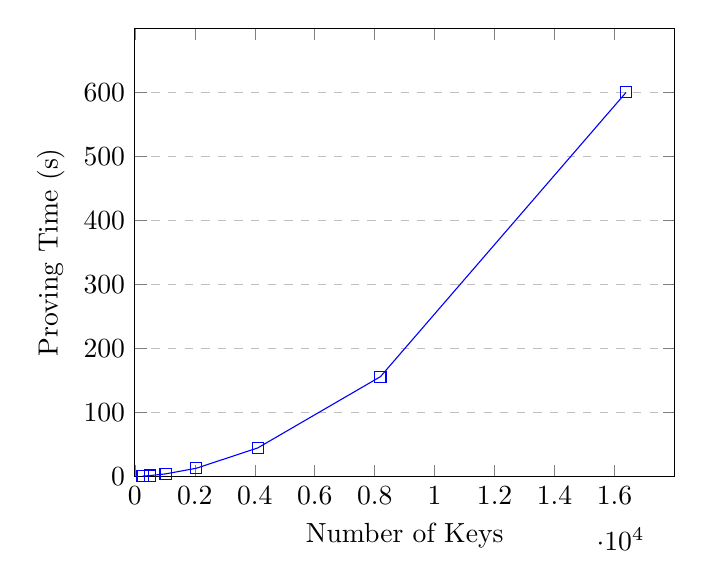
\begin{tikzpicture}
                \begin{axis}[
                    xlabel={Number of Keys},
                    ylabel={Proving Time (s)},
                    xmin=0,xmax=18000,
                    ymin=0,ymax=700,
                    xtick={0,2000,4000,6000,8000,10000,12000,14000,16000},
                    ytick={0,100,200,300,400,500,600},
                    ymajorgrids=true,
                    grid style=dashed,
                ]
                \addplot[
                    color=blue,
                    mark=square,
                ]
                    coordinates {
                        (256,0.63)(512,1.48)(1024,4.11)(2048,12.9)(4096,44.59)(8192,155.94)(16384,599.78)
                    };
                \end{axis}
            \end{tikzpicture}
        }
        \subcaption{}
    \end{subfigure}
    \begin{subfigure}{0.3\textwidth}
        \centering
        \resizebox{\linewidth}{!}{
            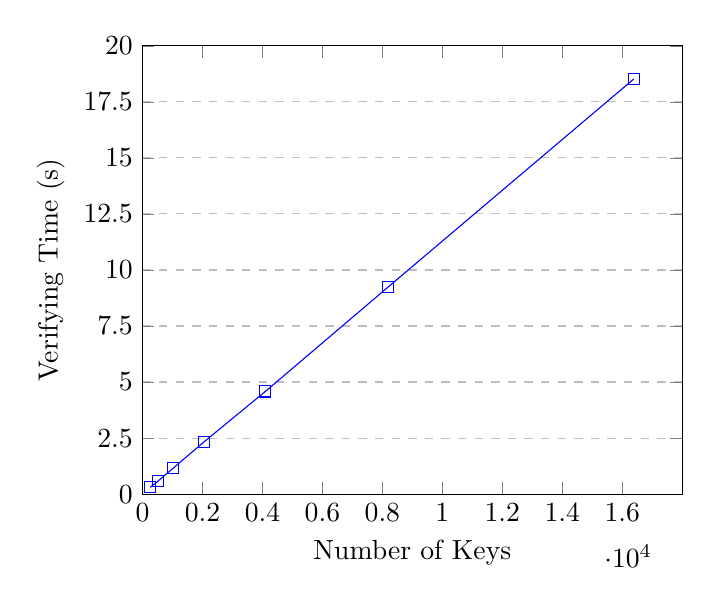
\begin{tikzpicture}
                \begin{axis}[
                    xlabel={Number of Keys},
                    ylabel={Verifying Time (s)},
                    xmin=0,xmax=18000,
                    ymin=0,ymax=20,
                    xtick={0,2000,4000,6000,8000,10000,12000,14000,16000},
                    ytick={0,2.5,5,7.5,10,12.5,15,17.5,20},
                    ymajorgrids=true,
                    grid style=dashed,
                ]
                \addplot[
                    color=blue,
                    mark=square,
                ]
                    coordinates {
                        (256,0.3)(512,0.58)(1024,1.16)(2048,2.33)(4096,4.58)(8192,9.24)(16384,18.52)
                    };
                \end{axis}
            \end{tikzpicture}
        }
        \subcaption{}
    \end{subfigure}
    \begin{subfigure}{0.3\textwidth}
        \centering
        \resizebox{\linewidth}{!}{
            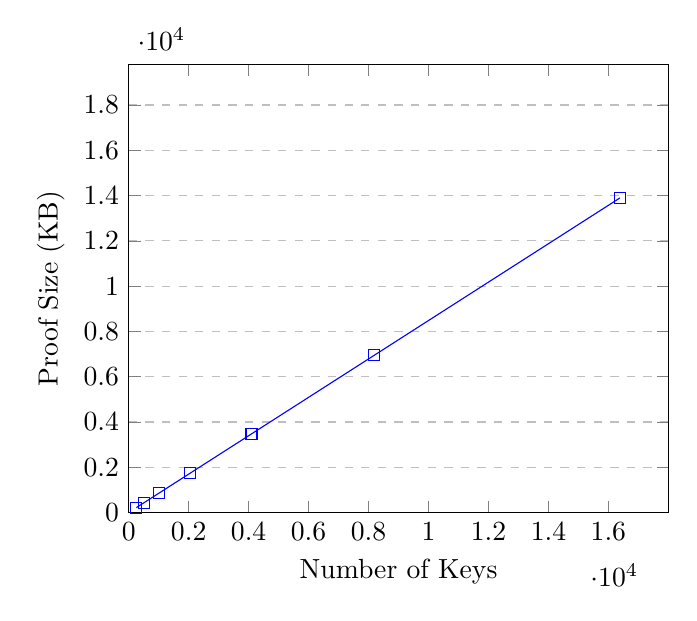
\begin{tikzpicture}
                \begin{axis}[
                    xlabel={Number of Keys},
                    ylabel={Proof Size (KB)},
                    xmin=0,xmax=18000,
                    ymin=0,ymax=19800,
                    xtick={0,2000,4000,6000,8000,10000,12000,14000,16000},
                    ytick={0,2000,4000,6000,8000,10000,12000,14000,16000,18000,20000},
                    ymajorgrids=true,
                    grid style=dashed,
                ]
                \addplot[
                    color=blue,
                    mark=square,
                ]
                    coordinates {
                        (256,217.0)(512,434.0)(1024,868.0)(2048,1736.0)(4096,3473.0)(8192,6946.0)(16384,13893.0)
                    };
                \end{axis}
            \end{tikzpicture}
        }
        \subcaption{}
    \end{subfigure}
\caption{Performance of \bootstrap. Subfigure (a) illustrates the number of keys and the proving time; Subfigure (b) and (c) indicate the verifying time and the proof size are linear in the number of keys.}
\end{figure*}

\begin{figure*}[t]
    \begin{subfigure}{0.3\textwidth}
        \resizebox{\linewidth}{!}{
            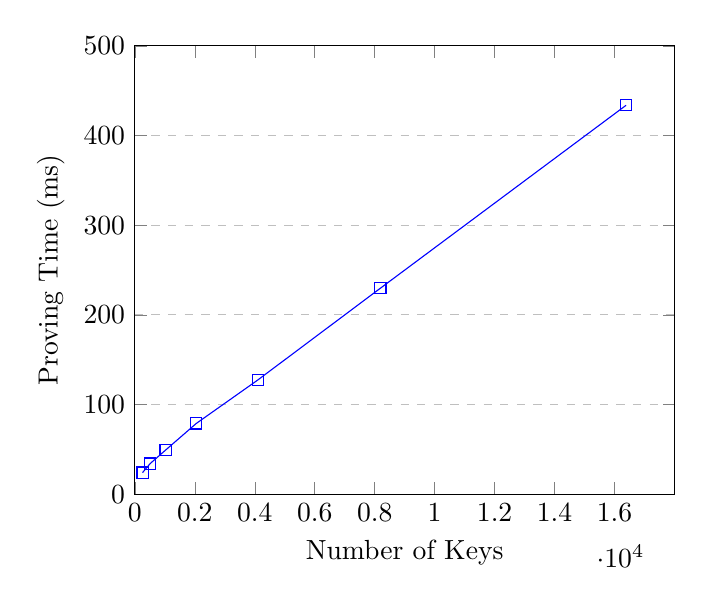
\begin{tikzpicture}
                \begin{axis}[
                    xlabel={Number of Keys},
                    ylabel={Proving Time (ms)},
                    xmin=0,xmax=18000,
                    ymin=0,ymax=500,
                    xtick={0,2000,4000,6000,8000,10000,12000,14000,16000},
                    ytick={0,100,200,300,400,500},
                    ymajorgrids=true,
                    grid style=dashed,
                ]
                \addplot[
                    color=blue,
                    mark=square,
                ]
                    coordinates {
                        (256,24.02)(512,34.1)(1024,49.09)(2048,78.8)(4096,127.17)(8192,229.71)(16384,433.66)
                    };
                \end{axis}
            \end{tikzpicture}
        }
        \subcaption{}
    \end{subfigure}
    \begin{subfigure}{0.3\textwidth}
        \resizebox{\linewidth}{!}{
            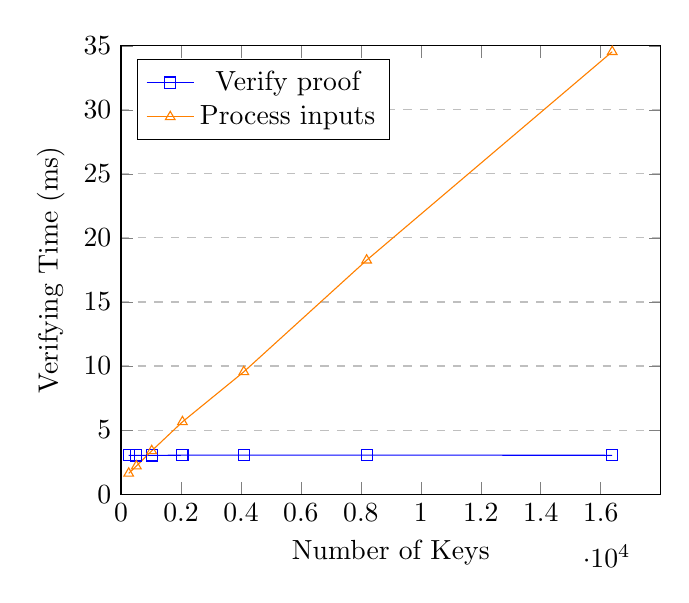
\begin{tikzpicture}
                \begin{axis}[
                    xlabel={Number of Keys},
                    ylabel={Verifying Time (ms)},
                    xmin=0,xmax=18000,
                    ymin=0,ymax=35,
                    xtick={0,2000,4000,6000,8000,10000,12000,14000,16000},
                    ytick={0,5,10,15,20,25,30,35},
                    ymajorgrids=true,
                    grid style=dashed,
                    legend pos=north west,
                ]
                \addplot[
                    color=blue,
                    mark=square,
                ]
                    coordinates {
                        (256,3.03)(512,3.02)(1024,3.02)(2048,3.04)(4096,3.04)(8192,3.05)(16384,3.03)
                    };
                \addlegendentry{Verify proof}

                \addplot[
                    color=orange,
                    mark=triangle,
                ]
                    coordinates {
                        (256,1.62)(512,2.19)(1024,3.38)(2048,5.64)(4096,9.55)(8192,18.26)(16384,34.54)
                    };
                \addlegendentry{Process inputs}
                \end{axis}
            \end{tikzpicture}
        }
        \subcaption{}
    \end{subfigure}
    \begin{subfigure}{0.3\textwidth}
        \resizebox{\linewidth}{!}{
            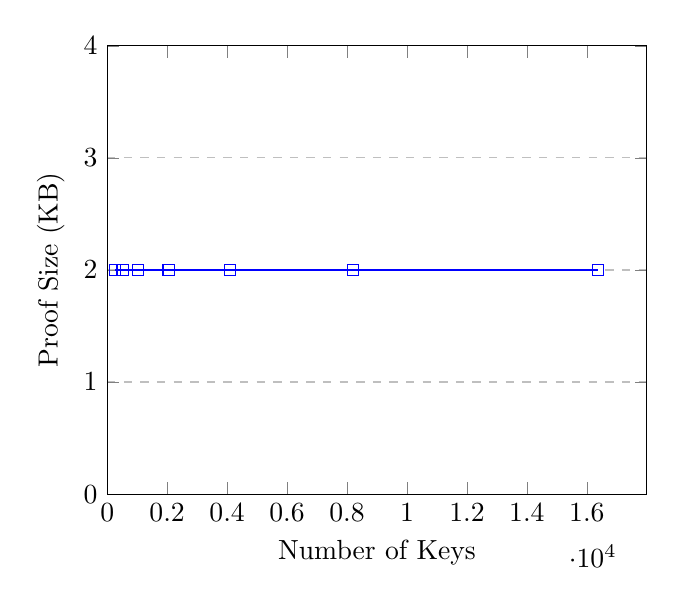
\begin{tikzpicture}
                \begin{axis}[
                    xlabel={Number of Keys},
                    ylabel={Proof Size (KB)},
                    xmin=0,xmax=18000,
                    ymin=0,ymax=4,
                    xtick={0,2000,4000,6000,8000,10000,12000,14000,16000},
                    ytick={0,1,2,3,4},
                    ymajorgrids=true,
                    grid style=dashed,
                ]
                \addplot[
                    color=blue,
                    mark=square,
                ]
                    coordinates {
                        (256,2.0)(512,2.0)(1024,2.0)(2048,2.0)(4096,2.0)(8192,2.0)(16384,2.0)
                    };
                \end{axis}
            \end{tikzpicture}
        }
        \subcaption{}
    \end{subfigure}
\caption{Performance of \poa. Subfigure (a) and (b) suggest the proving time and the verifying time are linear in the number of keys; Subfigure (c) shows the proof size is constant, 2KB, based on our implementation.}
\end{figure*}

\begin{figure*}[t]
    \begin{subfigure}{0.5\textwidth}
        \resizebox{\linewidth}{!}{
            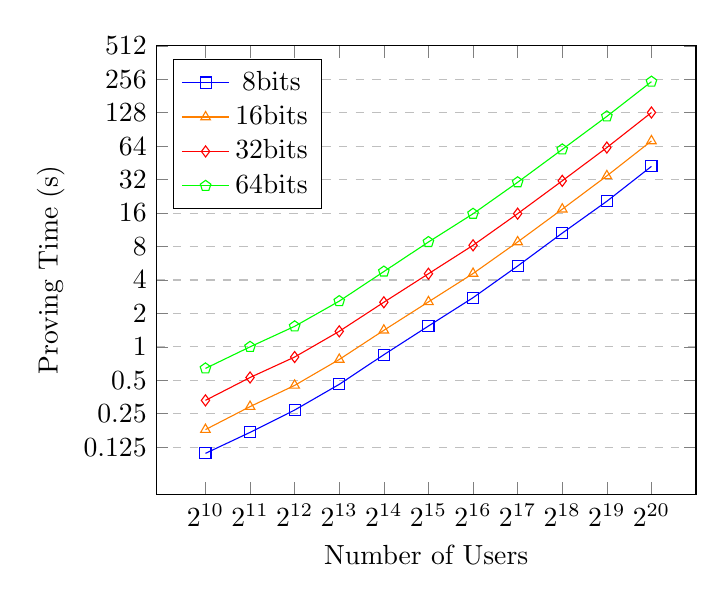
\begin{tikzpicture}
                \begin{loglogaxis}[
                    xlabel={Number of Users},
                    ylabel={Proving Time (s)},
                    xmin=0,xmax=2097152,
                    ymin=0,ymax=512,
                    xtick={0,1024,2048,4096,8192,16384,32768,65536,131072,262144,524288,1048576},
                    ytick={0,0.125,0.25,0.5,1,2,4,8,16,32,64,128,256,512},
                    xticklabels={$2^{10}$,$2^{11}$,$2^{12}$,$2^{13}$,$2^{14}$,$2^{15}$,$2^{16}$,$2^{17}$,$2^{18}$,$2^{19}$,$2^{20}$},
                    yticklabels={0.125,0.25,0.5,1,2,4,8,16,32,64,128,256,512},
                    ymajorgrids=true,
                    grid style=dashed,
                    legend pos=north west,
                ]
                \addplot[
                    color=blue,
                    mark=square,
                ]
                    coordinates {
                        (1024,0.11)(2048,0.17)(4096,0.27)(8192,0.46)(16384,0.85)(32768,1.54)(65536,2.77)(131072,5.34)(262144,10.56)(524288,20.43)(1048576,42.1)
                    };
                \addlegendentry{8bits}

                \addplot[
                    color=orange,
                    mark=triangle,
                ]
                    coordinates {
                        (1024,0.18)(2048,0.29)(4096,0.45)(8192,0.77)(16384,1.41)(32768,2.54)(65536,4.57)(131072,8.79)(262144,17.33)(524288,34.56)(1048576,71.31)
                    };
                \addlegendentry{16bits}

                \addplot[
                    color=red,
                    mark=diamond,
                ]
                    coordinates {
                        (1024,0.33)(2048,0.53)(4096,0.81)(8192,1.38)(16384,2.52)(32768,4.55)(65536,8.2)(131072,15.8)(262144,31.19)(524288,62.16)(1048576,128.49)
                    };
                \addlegendentry{32bits}

                \addplot[
                    color=green,
                    mark=pentagon,
                ]
                    coordinates {
                        (1024,0.64)(2048,1.0)(4096,1.53)(8192,2.58)(16384,4.76)(32768,8.78)(65536,15.76)(131072,30.27)(262144,59.8)(524288,118.57)(1048576,243.53)
                    };
                \addlegendentry{64bits}

                \end{loglogaxis}
            \end{tikzpicture}
        }
        \subcaption{}
    \end{subfigure}
    \begin{subfigure}{0.5\textwidth}
        \resizebox{\linewidth}{!}{
            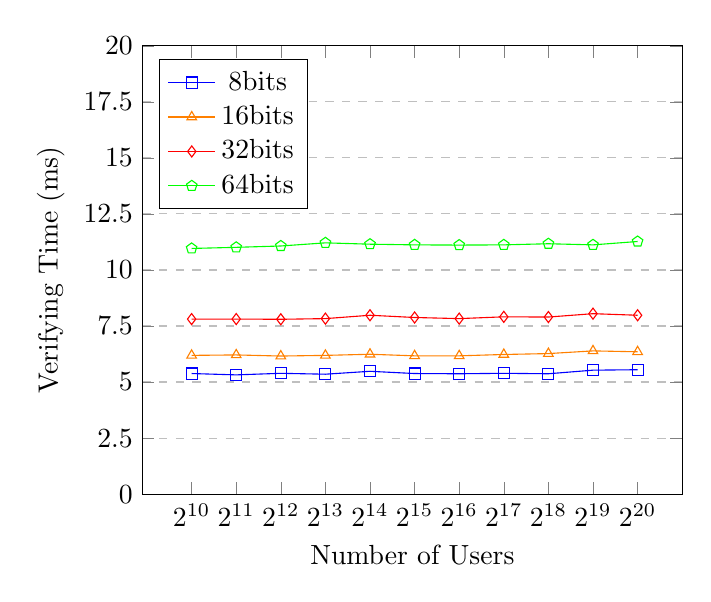
\begin{tikzpicture}
                \begin{semilogxaxis}[
                    xlabel={Number of Users},
                    ylabel={Verifying Time (ms)},
                    xmin=0,xmax=2097152,
                    ymin=0,ymax=20.0,
                    xtick={0,1024,2048,4096,8192,16384,32768,65536,131072,262144,524288,1048576},
                    ytick={0,2.5,5.0,7.5,10.0,12.5,15.0,17.5,20.0},
                    xticklabels={$2^{10}$,$2^{11}$,$2^{12}$,$2^{13}$,$2^{14}$,$2^{15}$,$2^{16}$,$2^{17}$,$2^{18}$,$2^{19}$,$2^{20}$},
                    ymajorgrids=true,
                    grid style=dashed,
                    legend pos=north west,
                ]

                \addplot[
                    color=blue,
                    mark=square,
                ]
                    coordinates {
                        (1024,5.38)(2048,5.32)(4096,5.39)(8192,5.35)(16384,5.48)(32768,5.38)(65536,5.37)(131072,5.39)(262144,5.37)(524288,5.53)(1048576,5.55)
                    };
                \addlegendentry{8bits}

                \addplot[
                    color=orange,
                    mark=triangle,
                ]
                    coordinates {
                        (1024,6.19)(2048,6.21)(4096,6.16)(8192,6.19)(16384,6.24)(32768,6.17)(65536,6.17)(131072,6.23)(262144,6.27)(524288,6.39)(1048576,6.35)
                    };
                \addlegendentry{16bits}

                \addplot[
                    color=red,
                    mark=diamond,
                ]
                    coordinates {
                        (1024,7.81)(2048,7.81)(4096,7.8)(8192,7.83)(16384,7.98)(32768,7.88)(65536,7.83)(131072,7.91)(262144,7.9)(524288,8.05)(1048576,7.98)
                    };
                \addlegendentry{32bits}

                \addplot[
                    color=green,
                    mark=pentagon,
                ]
                    coordinates {
                        (1024,10.96)(2048,11.01)(4096,11.07)(8192,11.21)(16384,11.15)(32768,11.12)(65536,11.11)(131072,11.12)(262144,11.17)(524288,11.12)(1048576,11.27)
                    };
                \addlegendentry{64bits}

                \end{semilogxaxis}
            \end{tikzpicture}
        }
        \subcaption{}
    \end{subfigure}

    \begin{subfigure}{0.5\textwidth}
        \resizebox{\linewidth}{!}{
            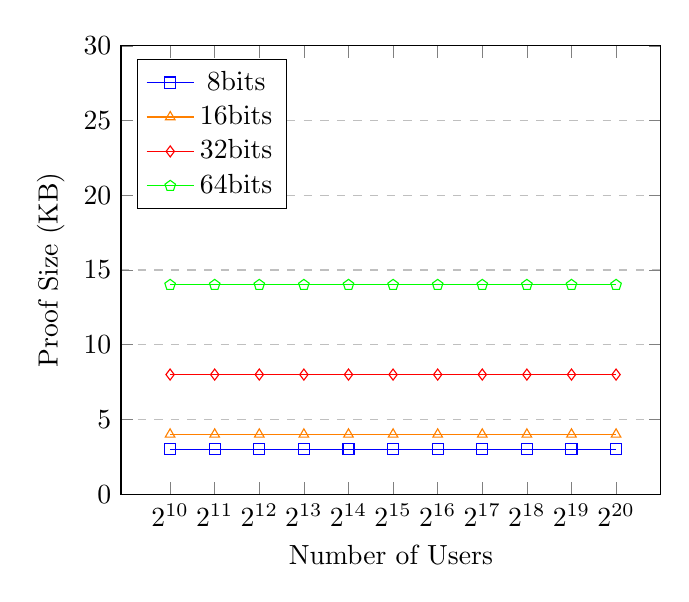
\begin{tikzpicture}
                \begin{semilogxaxis}[
                    xlabel={Number of Users},
                    ylabel={Proof Size (KB)},
                    xmin=0,xmax=2097152,
                    ymin=0,ymax=30,
                    xtick={0,1024,2048,4096,8192,16384,32768,65536,131072,262144,524288,1048576},
                    ytick={0,5,10,15,20,25,30},
                    xticklabels={$2^{10}$,$2^{11}$,$2^{12}$,$2^{13}$,$2^{14}$,$2^{15}$,$2^{16}$,$2^{17}$,$2^{18}$,$2^{19}$,$2^{20}$},
                    ymajorgrids=true,
                    grid style=dashed,
                    legend pos=north west,
                ]

                \addplot[
                    color=blue,
                    mark=square,
                ]
                    coordinates {
                        (1024,3.0)(2048,3.0)(4096,3.0)(8192,3.0)(16384,3.0)(32768,3.0)(65536,3.0)(131072,3.0)(262144,3.0)(524288,3.0)(1048576,3.0)
                    };
                \addlegendentry{8bits}

                \addplot[
                    color=orange,
                    mark=triangle,
                ]
                    coordinates {
                        (1024,4.0)(2048,4.0)(4096,4.0)(8192,4.0)(16384,4.0)(32768,4.0)(65536,4.0)(131072,4.0)(262144,4.0)(524288,4.0)(1048576,4.0)
                    };
                \addlegendentry{16bits}

                \addplot[
                    color=red,
                    mark=diamond,
                ]
                    coordinates {
                        (1024,8.0)(2048,8.0)(4096,8.0)(8192,8.0)(16384,8.0)(32768,8.0)(65536,8.0)(131072,8.0)(262144,8.0)(524288,8.0)(1048576,8.0)
                    };
                \addlegendentry{32bits}

                \addplot[
                    color=green,
                    mark=pentagon,
                ]
                    coordinates {
                        (1024,14.0)(2048,14.0)(4096,14.0)(8192,14.0)(16384,14.0)(32768,14.0)(65536,14.0)(131072,14.0)(262144,14.0)(524288,14.0)(1048576,14.0)
                    };
                \addlegendentry{64bits}

                \end{semilogxaxis}
            \end{tikzpicture}
        }
        \subcaption{}
    \end{subfigure}
\caption{Performance of PoL by different number of bits for the range proof. Subfigure (a) illustrates the proving time linearly relates to the number of users, and it is also linear to the number of bits for the same number of users; Subfigure (b) and (c) show the verifying time and the proof size are unrelated to the number of users, but relate to the number of bits. Unlike the proving time, the verifying time and the proof size do not linearly increase following the number of bits.\label{fig:pol}}
\end{figure*}


To evaluate the performance of \Sys, we implemented our protocols in Rust based on the popular library, arkworks\footnote{\url{https://github.com/arkworks-rs}}. Our implementation is publicly accessible on GitHub\footnote{GitHub: link removed for anonymity. Can supply code via the program chairs as necessary.}. We chose the pairing-friendly elliptic curve \bls for the KZG commitment which has 128 bit security.

Our experiments were conducted on a personal computer with i9-13900KF and 32GB of memory. The experimental data including balances and \secp key pairs are randomly generated locally for simplicity. Since there is no range-proof for PoA, we tested the PoA with balances randomly distributed in $[1,2^{64})$ to simulate the real distrbution of assets, and for PoL, we tested the program with balances randomly distributed in $[1,2^8)$, $[1,2^{16})$, $[1,2^{32})$, and $[1,2^{64})$. We simulated $2^8,2^9\dots,2^{14}$ and $2^{10},2^{11},\dots,2^{20}$ users for PoA and PoL respectively. Simulating different number of users for PoA and PoL is because \bootstrap was time-consuming for larger number of users. For each protocol, we ran the test for ten times with the same experimental data. Our figures are interpolated from the average performance of ten times while discarding the maximum and the minimum samples.

\subsection{Experimental Evaluation}
Figure 2, 3, and 4 reflect the performance of \Sys in single thread with i9-13900KF. We discarded the samples of the maximum and the minimum to calculate the average for each point. The Subfigure (a) of Figure 2 suggests it takes around 600 seconds to generate the proofs for 16,384 keys with i9-13900KF for \bootstrap, and the proof size is 13,893KB. There are around $2^{28}$ unique Ethereum addresses reported by Ethercan.io in May 2024 \footnote{\url{https://etherscan.io/chart/address}}, which means it requires 9,830,400 computing instances to generate the proofs for all the keys in 600 seconds if the exchange wants the maximum anonymous set. It seems impractical for the exchange to depoly such number of servers in the real world. However, recall the exchange only needs to perform \bootstrap once. The exchange can sacrifice the proving time to reduce the number of servers. Moreover, the proving time can be reduced significantly if manipulating more efficient KZG opening schemes. See Section~\ref{sec:opt} for more detailed optimizations. 

Figure 3 shows the proving time and the verifying time are linear in the number of the keys. In our experiments, it takes 433.66 milliseconds to generate the proof and 37.57 milliseconds to verify the proof for 16,384 keys. This suggests the proving time is less than 2 hours if the anonymous set is the whole addresses on Ethereum without any other optimizations! Since the proof size of a KZG commitment is unrelated to the degree of the polynomial (the number of keys), the proof size of \poa is 2KB based on our implementation.

Figure 4 illustrates the performance of our PoL with different number of users and allowed ranges for balance. Our experiments show the proving time grows linearly with the number of users while the verifying time and the proof size are constant. From the test result of Binance's PoL, it needs 1.5 days to generate the proof for 100 million accounts with 100 servers \footnote{\url{https://github.com/binance/zkmerkle-proof-of-solvency/?tab=readme-ov-file}}, but our PoL requires less than 10 minutes with the same number of servers! This indicates our protocol is practical to handle the real-world applications.

\subsection{Optimization}
\label{sec:opt}
Due to the additively homomorphic property of KZG commitment, the prover's work in our protocols can be easily splitted to arbitrary number of servers, and there is no need to provide extra proofs to aggregate the proofs from different servers (provers). That means the proving time will decrease with the growing number of servers. This is the most direct method to make the protocols more efficient. Another way to improve the performance without adding more servers is utilizing more efficient KZG opening schemes. Recall the heaviest work of \bootstrap is proving each committed point is correct, and the opening scheme we demonstrated from Plonk requires $t\cdot{d}$ scalar multiplications for prover, where $t$ is the number of the opening points and $d$ is the degree bound of the polynomial. The work in BDFG20~\cite{bdfg} can reduce this complexity to $2n$ scalar multiplications, which means the dominating complexity will become $O(n)$ rather than $O(n^2)$. The aggreation slightly increases the verifier's work but the extra cost is trivial because of the succinctness of KZG commitment scheme. These optimizations can be applied to both of our PoA and PoL. Moreover, the proof length for multiple points of the KZG commitment will also be decreased to $O(1)$ if BDFG20 is intergated, but the total proof length is still $O(n)$ because of the proof of the $\Sigma$-protocol.



% = = = = = = = = = = = = = = = = = = = = = = = = = = = = = = = = = = =


\section{Open Research Challenges}

We presented \Sys as a Poly-IOP solvency argument. The efficiency and succinctness of \Sys might be further improved using advances in other poly-iop systems: lookup arguments and multivariate polynomials (and corresponding commitment schemes). Techniques from recursive SNARKs might enable solvency proofs that are repeated (say every day) to reduce prover time by ignoring ETH addresses and user balances that did not change across the day, while still allowing a verifier to have full confidence in the history of the exchange if they only check the most recent proof. If blockchains like Ethereum add low-gas cost support for \bls, a topic of discussion (EIP-2537\footnote{\url{https://eips.ethereum.org/EIPS/eip-2537}}), verifying proofs of solvency could move on-chain. If an exchange fails to provide a smart contract with a proof of solvency in a timely fashion, the smart contract could be called to trigger penalties or other actions. 

Standardization work could also be useful for proofs of solvency. Of the exchanges that opt into providing proofs of solvency, the exact protocol can vary from other exchanges, and it is not always deployed correctly (at least initially)~\cite{broken}. Having the community coalesce behind a proof template, working out every detail, with audited and formally verified reference code could be helpful to exchanges. \Sys is a good start as it is a complete end-to-end proof system, and is competitive in prover time, verifier time and proof size with other sub-components introduced in the literature.

 
% = = = = = = = = = = = = = = = = = = = = = = = = = = = = = = = = = = = = = = = = = =

\paragraph{Scope.} 
Blah blah blah.

% = = = = = = = = = = = = = = = = = = = = = = = = = = = = = = = = = = = = = = = = = =

\paragraph{Contributions.} 
Our primary contributions are as follows.

\begin{enumerate}

\item Blah blah blah.

\item Blah blah blah. 

\item Blah blah blah. 

\end{enumerate}

